\chapter{Análisis y diseño}
    \label{chap:four}

\renewcommand{\labelitemi}{$\bullet$}
\renewcommand{\labelitemii}{$\circ$}
\renewcommand{\labelitemiii}{$\Rightarrow$}

\section{¿Qué es un agente?}
A lo largo de las últimas décadas, la definición de agente se ha ido completando y adaptando para con la evolución. 
\newline La primera definición se construye en base a las principales características de \textbf{autonomía} e \textbf{inteligencia}. De este periodo son las arquitecturas deliberativas y reactivas en base a las cuales estaban construidos agentes sencillos de acción-reacción.
\newline Posteriormente, con la extensión de internet y las posibilidades que este ofrece, los agentes evolucionan a un modelo \textbf{comunicativo}, manteniendo las características ya conocidas. En este punto, aparecen agentes móviles que se comunican gracias a implementación de estándares.
\newline Más tarde, se dota a los agentes de una \textbf{dimensión social}. A partir de aquí, los agentes se crean teniendo en cuenta modelos sociales reales con mecanismos de interacción, toma de decisiones, posesión de sentimientos, aprendizaje, etc.

Un \textbf{agente} es un sistema computacional establecido en un entorno y con la capacidad de actuar de forma autónoma para la consecución de sus propios objetivos.

Un \textbf{sistema multiagente} es un conjunto de agentes que interactúan entre sí con el fin de conseguir objetivos propios y/o comunes, para lo cual, entre otras cosas, necesitan realizar acciones comunicativas, cooperativas, de coordinación y de negociación.
\newline \cite{dba2122, intelligent_agents}

\newpage
\subsection{Estructura de un agente}
Los agentes inteligentes poseen un ciclo de vida. Un ciclo de vida de un agente implementado usando el framework \acrshort{jade}, de forma simplificada, está compuesto por la siguientes fases: creación, realización de acciones y destrucción.
\begin{enumerate}
    \item \textbf{Inicialización del agente}, método \lstinline{setup()}. Se crean e inicializan todos los atributos necesarios para el correcto funcionamiento del agente.
    \item \textbf{Realización de acciones}, método \lstinline{execute()}. Se ejecutan determinadas acciones mientras el agente esté activo. De forma resumida, esta fase se estructura como un bucle condicional basado en una condición de finalización. Las acciones se repiten mientras el bucle no finalice, es decir, mientras que la condición de finalización no se cumpla.
    \item \textbf{Finalización del agente}, método \lstinline{takeDown()}. Se finaliza la ejecución. Terminan todos los procesos relativos a la ejecución (vida) del agente.
\end{enumerate}

\subsection{Comunicación entre agentes}
En \acrshort{jade}, los agentes pueden comunicarse de forma transparente independientemente de si viven en el mismo contenedor, en diferentes contenedores pertenecientes a la misma plataforma o en diferentes plataformas. La comunicación se basa en un paradigma de paso de mensajes asíncrono. El formato de los mensajes está definido por el lenguaje \acrfull{acl} definido por la \acrfull{fipa}, una organización internacional que emitió un conjunto de especificaciones para la interoperabilidad de los agentes.

Un mensaje \acrshort{acl} está constituido por una serie de parámetros: sender, receiver, content, reply\_with, in\_reply\_to, encoding, language, ontology, reply\_by, protocol, conversation\_id y performative, entre los cuales:
\begin{itemize}
    \item \textbf{Sender}: el identificador del agente que envía el mensaje.
    \item \textbf{Receiver}: los identificadores de los agentes que reciben el mensaje (el mensaje puede ser recibido por uno o varios agentes).
    \item \textbf{Content}: el contenido del mensaje. Es una cadena, por lo tanto, se pueden enviar mensajes codificados de diferente forma (para lo cual sería necesario indicarlo en el parámetro \textit{encoding}).
    \item \textbf{Conversation-id}: el identificador de la conversación entre los agentes.
    \item \textbf{Performative}: el tipo de acto comunicativo, es decir, el tipo de acción que se realiza (la interpretación que se le da).
\end{itemize}
 Existen diferentes tipos de actos comunicativos, es decir, de performativas: accept-proposal, agree, cancel, cfp, confirm, disconfirm, failure, refuse, reject-proposal, request, request-when, request-whenever, subscribe, inform, inform-if, inform-ref, not-understood, propose, query-if y query-ref, entre las cuales:
 \begin{itemize}
     \item \textbf{REQUEST}: El \textit{sender} pide a los \textit{receivers} que ejecuten una acción. Entre las performativas posibles para las respuestas asociadas al envío de un mensaje con esta performativa se encuentran: inform, refuse, agree, failure y not-understood.
     \item \textbf{SUBSCRIBE}: El \textit{sender} se suscribe al \textit{receiver} para con los cambios del valor de un objeto. Se aplica el patrón \textit{observer}. Entre las performativas posibles para las respuestas asociadas al envío de un mensaje con esta performativa se encuentran: inform y refuse.
     \item \textbf{INFORM}: El \textit{sender} informa de algo a los \textit{receivers}. Tiene multitud de implicaciones y, generalmente, se utiliza en mensajes de respuesta.
 \end{itemize}
 

\cite{dba2122, fipa}

\newpage
\section{Planteamiento del problema}
%
% ¿POr qué es importante controlar mejor el tráfico? ¿Qué problemas implica? ¿Cómo están resueltas en la literatura? ¿Cómo pretendes abordarla tu? ¿ Por qué? ¿Cómo vas a evaluar las soluciones que propones? ¿Por qué?
%
    \label{section:problem}
La construcción de un sistema multiagente para el control del tráfico es algo complicado, sin embargo, no es necesario abordar todos las casuísticas que se plantean con respecto a este tema desde un principio. Con las tecnologías que se tienen en el momento, es seguro que existen un gran cantidad de formas diferentes de abordar este reto.

Intentar construir el sistema completo, desde un inicio y con toda su complejidad, podría ser abrumador. Por ello, es necesario dividir el problema en pequeñas partes que ir abordando de forma individual hasta la consecución de los objetivos planteados. Esta es la filosofía a seguir.

Además de dividir en pequeñas tareas, es necesario definir un conjunto de simplificaciones para la construcción del sistema. Son las siguientes:
\begin{itemize}
    \item \textbf{Modelos simple y estándar de cruce}. Desde un modelo de cruce simple se evolucionará a un modelo de cruce estándar. Se modelarán cruces cuya representación sea posible en base al modelo planteado para los tipos de cruce mencionados. Hay que tener muy en cuenta que el sistema construido debe ser escalable, es decir, su arquitectura debe permitir representar diferentes escenarios de forma eficaz, desde los más triviales hasta los más complejos.
    \item \textbf{Tiempo de ciclo fijo}. El tiempo que dura el paso entre todos los estados de un cruce es fijo, es decir, el tiempo que pasa desde que un cruce inicia en un estado hasta que vuelve a ese mismo estado habiendo pasado por todos los demás.
    \item \textbf{Los semáforos únicamente regulan la entrada al cruce, no la salida}. No existen semáforos que no estén dedicados exclusivamente a regular la entrada de tráfico a un cruce.
    \item \textbf{Los vehículos tardan un instante en pasar el cruce}. Los vehículos tardan un segundo en ir desde un tramo de calle origen hasta otro tramo de calle destino a través del cruce, es decir, tardan un segundo en recorrer un tramo de cruce.
    \item \textbf{No existen aparcamientos, es decir, todo vehículo que entra al sistema sale de él}. En el sistema entran y salen vehículos. Ningún vehículo puede permanecer en el sistema al final de una simulación a no ser que no le haya dado tiempo a ir desde la entrada hasta una salida.
    \item \textbf{No existen ni peatones ni metro ni ningún tipo de infraestructura asociada a los mismos}. Los peatones no se contemplan en el sistema \acrshort{murat}, para el sistema no existen.
\end{itemize}

Teniendo en cuenta las simplificaciones planteadas, se va a obtener la información funcional necesaria para construir el sistema a través de diferentes preguntas.

Una pregunta muy importante a responder es: \textit{¿qué se quiere representar?} Simplificando, se quieren representar dos cosas:
\begin{itemize}
    \item el \textbf{lugar físico} (el mundo) por donde circulan los vehículos: calles, cruces y semáforos;
    \item y el propio \textbf{tráfico}, el cual debe respetar sus propias reglas y las del lugar físico.
\end{itemize}

A partir de lo anterior, en relación al primer punto, surge la siguiente pregunta: \textit{¿qué es una ciudad, escenario, lugar físico o mundo para el sistema?} Es un conjunto de uno o más cruces que pueden ser: entradas al sistema, lugares internos al sistema y/o salidas del sistema. El modelo de ciudad es un grafo dirigido donde los nodos son las calles y las aristas las conexiones entre las mismas. En este momento aparece otra pregunta: \textit{¿qué elementos forman una ciudad y sus cruces, es decir, el entorno?} El entorno está formado por los siguientes elementos:
\begin{itemize}
    \item \textbf{Ciudad/Escenario}: Es el entorno del sistema.
    \begin{itemize}
        \item \textbf{Tramo de calle}: Es cada una de las partes de una calle en la que los vehículos circulan en un sentido. Puede estar constituido por uno o varios carriles. Sirve de entrada al sistema, de conexión entre dos cruces o de salida del sistema. En la figura \ref{fig:cruce_simple_topologia} son tramos de calle RS1, RS2, RS3 y RS4. Si el tramo de calle es de entrada al cruce está regulado por un semáforo. En la figura \ref{fig:cruce_simple_topologia} están regulados por semáforos los tramos de calle RS2, por TL1, y RS3, por TL2. \newline 
        Un tramo de calle tiene una longitud y un número de carriles. Con estos valores y una constante que define la longitud de los vehículos se puede calcular la capacidad máxima de vehículos de los tramos de calle. El porcentaje de ocupación de un tramo de calle es la relación existente entre la cantidad de vehículos del tramo de calle y la capacidad máxima de vehículos de ese tramo de calle.
        \item \textbf{Cruce}: Es una intersección de varias calles. Al cruce llegan tramos de calle y del cruce salen tramos de calle. Contiene semáforos que habilitan o no tramos de cruce para pasar de un lado a otro del cruce. En el sistema es un agente.
        \begin{itemize}
            \item \textbf{Semáforo}: Regula el tráfico de vehículos proveniente de un tramo de calle de entrada a un cruce. En el sistema es un agente.
            \item \textbf{Tramo de cruce}: Es cada uno de los recorridos que puede hacer un vehículo para pasar un cruce. Está definido por un tramo de calle de origen y un tramo de calle destino. En la figura \ref{fig:cruce_simple_estados_1y2} es un tramo de calle RS3-RS1.
            \item \textbf{Estado}: Define los colores de los semáforos y habilita determinados tramos de cruce. En la figura \ref{fig:cruce_simple_estados_1y2} se pueden ver dos estados para el mismo cruce. 
        \end{itemize}
    \end{itemize}
\end{itemize}

En este punto, en relación a la segunda cuestión, surge otra pregunta: \textit{¿cómo es añadido el tráfico al sistema?} El tráfico se añade a los tramos de calle que no tengan cruce de origen y tengan cruce de destino, es decir, los vehículos entran por los nodos raíz. Para saber el instante en el que añadir tráfico al sistema se utiliza una constante denominada ratio de entrada de tráfico al sistema. Si el tráfico entra, el tráfico tiene que salir, entonces: \textit{¿cómo sale el tráfico del sistema?} El tráfico sale del sistema por los tramos de calle que tienen cruce de origen pero no tienen cruce de destino, es decir, los vehículos salen por los nodos hoja. En relación a la entrada del tráfico, hay periodos del día, es decir, periodos de la simulación, donde la afluencia de tráfico es mayor. A esto se le denomina horas punta y se traduce en una mayor adición de vehículos al sistema.\newline
En relación al tráfico, también, es necesario preguntarse: \textit{¿qué vehículos van hacia qué tramo de calle en el cruce?} A priori, como no se sabe, se puede partir de un modelo equiprobable. En función de la capacidad de los tramos de calle girarán más o menos vehículos (si un tramo de calle tiene más capacidad se supone que es porque van a entrar más vehículos). En relación a lo anterior se establece la ratio de desvío, que es el porcentaje de vehículos que giran en los cruces a cada tramo de calle.

Una vez se ha explicado todo lo relacionado a la representación de la realidad en el sistema, es necesario hablar sobre lo que se quiere conseguir con \acrshort{murat}. El principal objetivo es aumentar el número de vehículos que pueden procesarse en una simulación, pero \textit{¿cómo se puede conseguir el objetivo principal del sistema?} Optimizando los tiempos de los estados de los cruces, beneficiando aquellos que permitan el paso de vehículos desde tramos de calle saturados. Es decir, aumentando el tiempo de los estados mencionados y disminuyendo el tiempo de los estados cuyos tramos de calle tengan menos ocupación, respetando el límite mínimo de tiempo de duración de un estado.

\newpage
\subsection{Cruce simple}
    \label{subsection:cruce_simple}
Lo que se puede apreciar en la figura \ref{fig:cruce_simple_topologia} es lo que se ha denominado como cruce simple. En este cruce se produce una intersección vial de dos calles: 
\begin{itemize}
    \item el flujo de tráfico de la primera de ellas, regulado por el semáforo \textbf{TL2} y representada por \textbf{RS3} y \textbf{RS1}, pasa por el cruce en sentido oeste a este; 
    \item y el flujo de tráfico de la segunda de ellas, regulado por el semáforo \textbf{TL1} y representada por \textbf{RS2} y \textbf{RS4} pasa por el cruce en sentido norte a sur.
\end{itemize}
\begin{figure}[H]
    \centering
    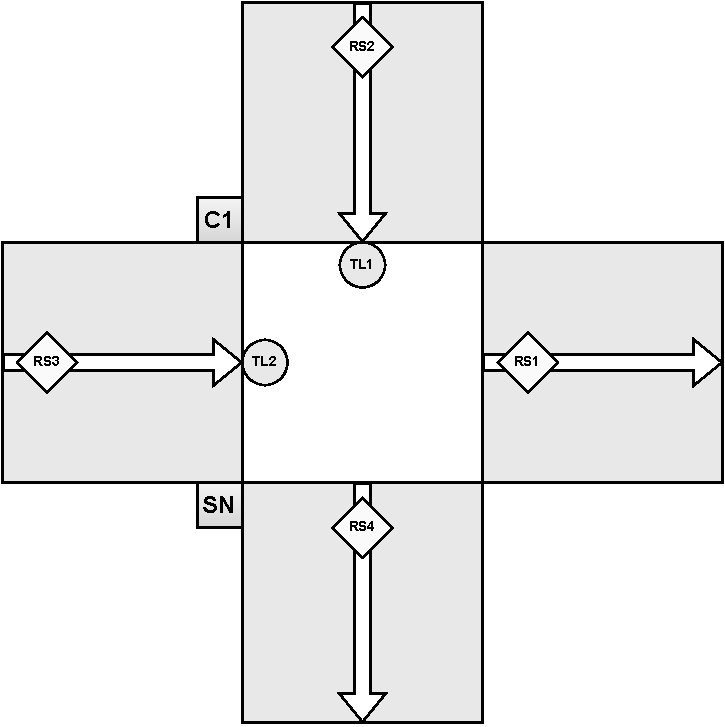
\includegraphics[width=0.75\linewidth]{text/image/DCruc-CS-Topologia.pdf}
    \caption{Topología del cruce simple}
    \label{fig:cruce_simple_topologia}
\end{figure}

\newpage
El cruce simple posee dos estados diferentes en función del color de los semáforos, los cuales habilitan o bloquean el tránsito de vehículos desde unos tramos de calle hasta otros.

El \textbf{primer estado}, expuesto en la figura \ref{fig:cruce_simple_estados_1y2}:
\begin{itemize}
    \item habilita el tránsito de vehículos desde el tramo de calle \textbf{RS2} hasta el tramo de calle \textbf{RS1} y desde el tramo de calle \textbf{RS2} hasta el tramo de calle \textbf{RS4}, es decir, habilita los tramos de cruce \textbf{RS2-RS1} y \textbf{RS2-RS4};
    \item y bloquea el tránsito de vehículos desde el tramo de calle \textbf{RS3} hasta el tramo de calle \textbf{RS1} y desde el tramo de calle \textbf{RS3} hasta el tramo de calle \textbf{RS4}, es decir, bloquea los tramos de cruce \textbf{RS3-RS1} y \textbf{RS3-RS4}.
\end{itemize}

El \textbf{segundo estado}, expuesto en la figura \ref{fig:cruce_simple_estados_1y2}:
\begin{itemize}
    \item habilita el tránsito de vehículos desde el tramo de calle \textbf{RS3} hasta el tramo de calle \textbf{RS1} y desde el tramo de calle \textbf{RS3} hasta el tramo de calle \textbf{RS4}, es decir, habilita los tramos de cruce \textbf{RS3-RS1} y \textbf{RS3-RS4};
    \item y bloquea el tránsito de vehículos desde el tramo de calle \textbf{RS2} hasta el tramo de calle \textbf{RS1} y desde el tramo de calle \textbf{RS2} hasta el tramo de calle \textbf{RS4}, es decir, bloquea los tramos de cruce \textbf{RS2-RS1} y \textbf{RS2-RS4}.
\end{itemize}

\begin{figure}[H]
    \centering
    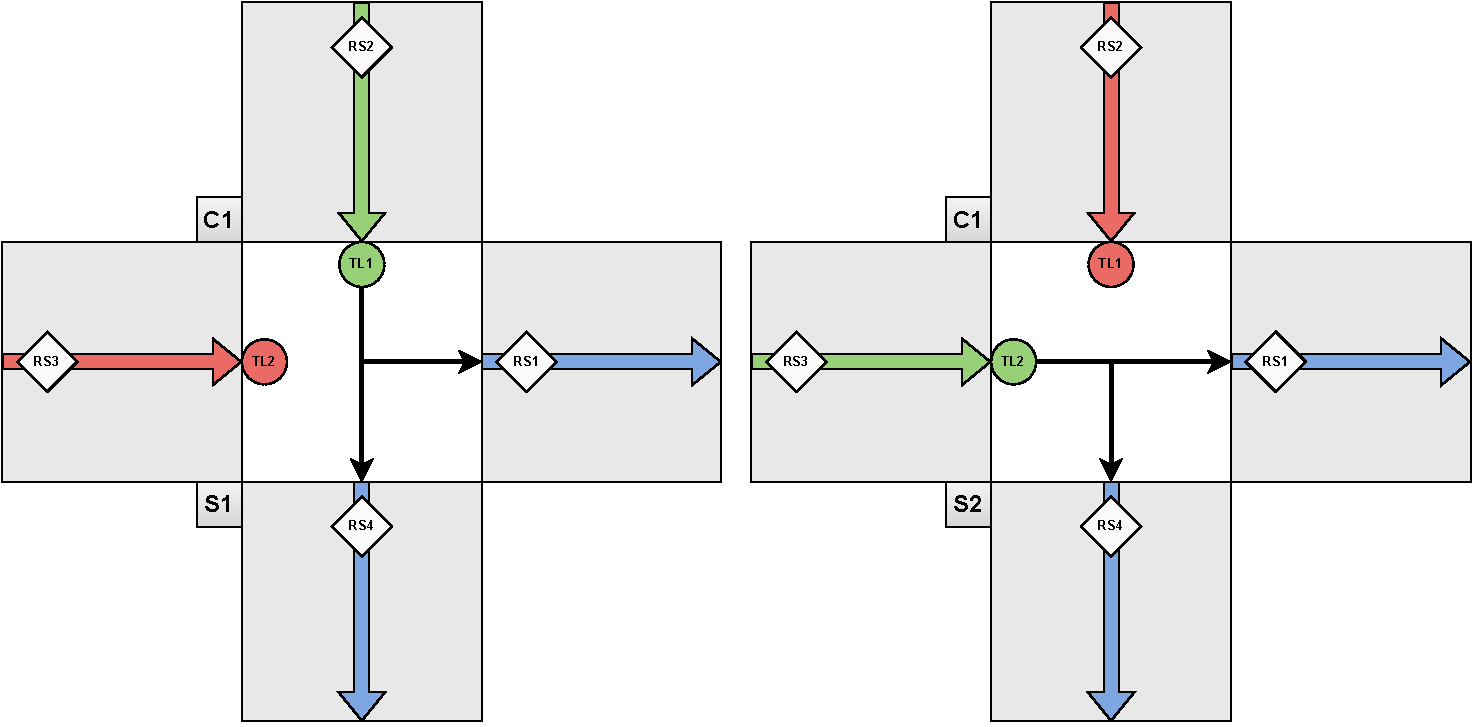
\includegraphics[width=1\linewidth]{text/image/DCruc-CS-Estados1y2.pdf}
    \caption{Cruce simple en estados 1 y 2}
    \label{fig:cruce_simple_estados_1y2}
\end{figure}

\newpage
\subsection{Cruce estándar}
    \label{subsection:cruce_estandar}
Lo que se puede apreciar en la figura \ref{fig:cruce_estandar_topologia} es lo que se ha denominado como cruce estándar. Como se puede observar, el cruce estándar posee una mayor complejidad, teniendo tramos de calle con flujo de coches en diferentes sentidos y varios carriles. En este cruce, también, se produce una intersección vial de dos calles: 
\begin{itemize}
    \item el flujo de tráfico de la primera de ellas, regulado por los semáforos \textbf{TL1} (entrada al cruce desde el este por \textbf{RS1}) y \textbf{TL3} (entrada al cruce desde el oeste por \textbf{RS5}); 
    \item y el flujo de tráfico de la segunda de ellas, regulado por los semáforos \textbf{TL2} (entrada al cruce desde el norte por \textbf{RS3}) y \textbf{TL4} (entrada al cruce desde el sur por \textbf{RS7}).
\end{itemize}

\begin{figure}[H]
    \centering
    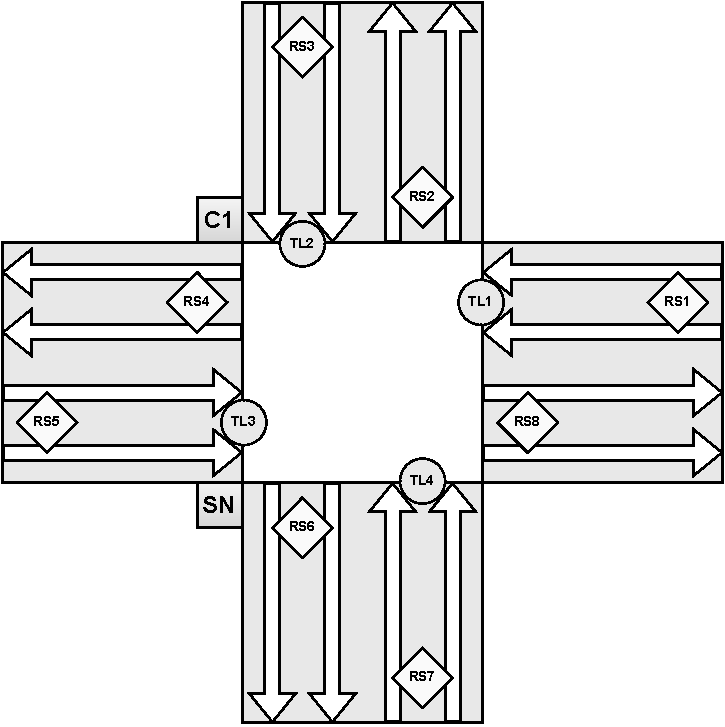
\includegraphics[width=0.75\linewidth]{text/image/DCruc-CE-Topologia.pdf}
    \caption{Topología del cruce estándar}
    \label{fig:cruce_estandar_topologia}
\end{figure}

\newpage
El cruce estándar posee seis estados diferentes en función del color de los semáforos, los cuales habilitan o bloquean el tránsito de vehículos desde unos tramos de calle hasta otros.

El \textbf{primer estado}, expuesto en la figura \ref{fig:cruce_estandar_estados_1y2}:
\begin{itemize}
    \item habilita el tránsito de vehículos desde el tramo de calle \textbf{RS3} hasta los tramos de calle \textbf{RS4} y \textbf{RS6} y desde el tramo de calle \textbf{RS7} hasta los tramos de calle \textbf{RS2} y \textbf{RS8}, es decir, habilita los tramos de cruce \textbf{RS3-RS4}, \textbf{RS3-RS6}, \textbf{RS7-RS2} y \textbf{RS7-RS8};
    \item y bloquea el tránsito de vehículos desde los tramos de calle \textbf{RS1} y \textbf{RS5}.
\end{itemize}

El \textbf{segundo estado}, expuesto en la figura \ref{fig:cruce_estandar_estados_1y2}:
\begin{itemize}
    \item habilita el tránsito de vehículos desde el tramo de calle \textbf{RS3} hasta los tramos de calle \textbf{RS4}, \textbf{RS6} y \textbf{RS8}, es decir, habilita los tramos de cruce \textbf{RS3-RS4}, \textbf{RS3-RS6} y \textbf{RS3-RS8};
    \item y bloquea el tránsito de vehículos desde los tramos de calle \textbf{RS1}, \textbf{RS5} y \textbf{RS7}.
\end{itemize}
\begin{figure}[H]
    \centering
    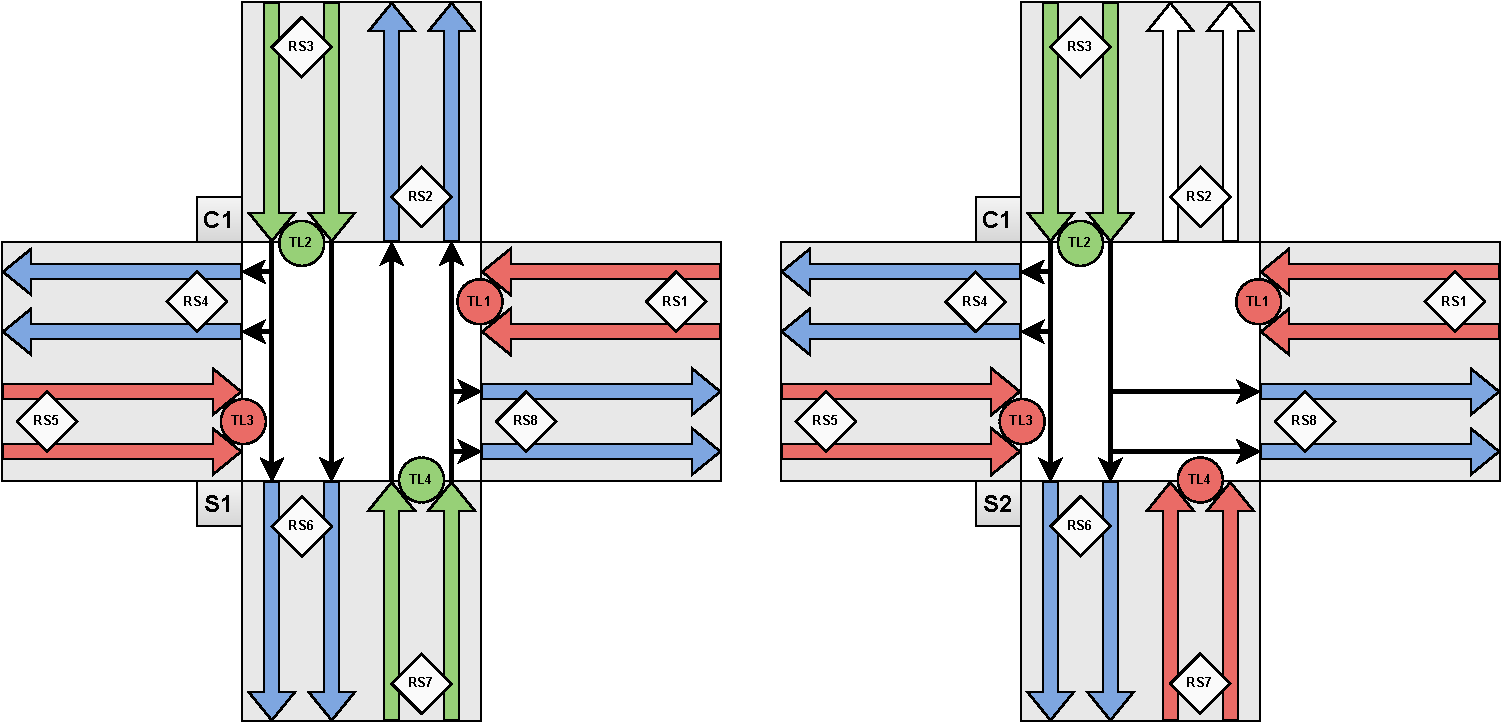
\includegraphics[width=1\linewidth]{text/image/DCruc-CE-Estados1y2.pdf}
    \caption{Cruce estándar en estados 1 y 2}
    \label{fig:cruce_estandar_estados_1y2}
\end{figure}

\newpage
El \textbf{tercer estado}, expuesto en la figura \ref{fig:cruce_estandar_estados_3y4}:
\begin{itemize}
    \item habilita el tránsito de vehículos desde el tramo de calle \textbf{RS7} hasta los tramos de calle \textbf{RS2}, \textbf{RS4} y \textbf{RS8}, es decir, habilita los tramos de cruce \textbf{RS7-RS2}, \textbf{RS7-RS4} y \textbf{RS7-RS8};
    \item y bloquea el tránsito de vehículos desde los tramos de calle \textbf{RS1}, \textbf{RS3} y \textbf{RS5}.
\end{itemize}

El \textbf{cuarto estado}, expuesto en la figura \ref{fig:cruce_estandar_estados_3y4}:
\begin{itemize}
    \item habilita el tránsito de vehículos desde el tramo de calle \textbf{RS1} hasta los tramos de calle \textbf{RS2} y \textbf{RS4} y desde el tramo de calle \textbf{RS5} hasta los tramos de calle \textbf{RS6} y \textbf{RS8}, es decir, habilita los tramos de cruce \textbf{RS1-RS2}, \textbf{RS1-RS4}, \textbf{RS5-RS6} y \textbf{RS5-RS8};
    \item y bloquea el tránsito de vehículos desde los tramos de calle \textbf{RS3} y \textbf{RS7}.
\end{itemize}
\begin{figure}[H]
    \centering
    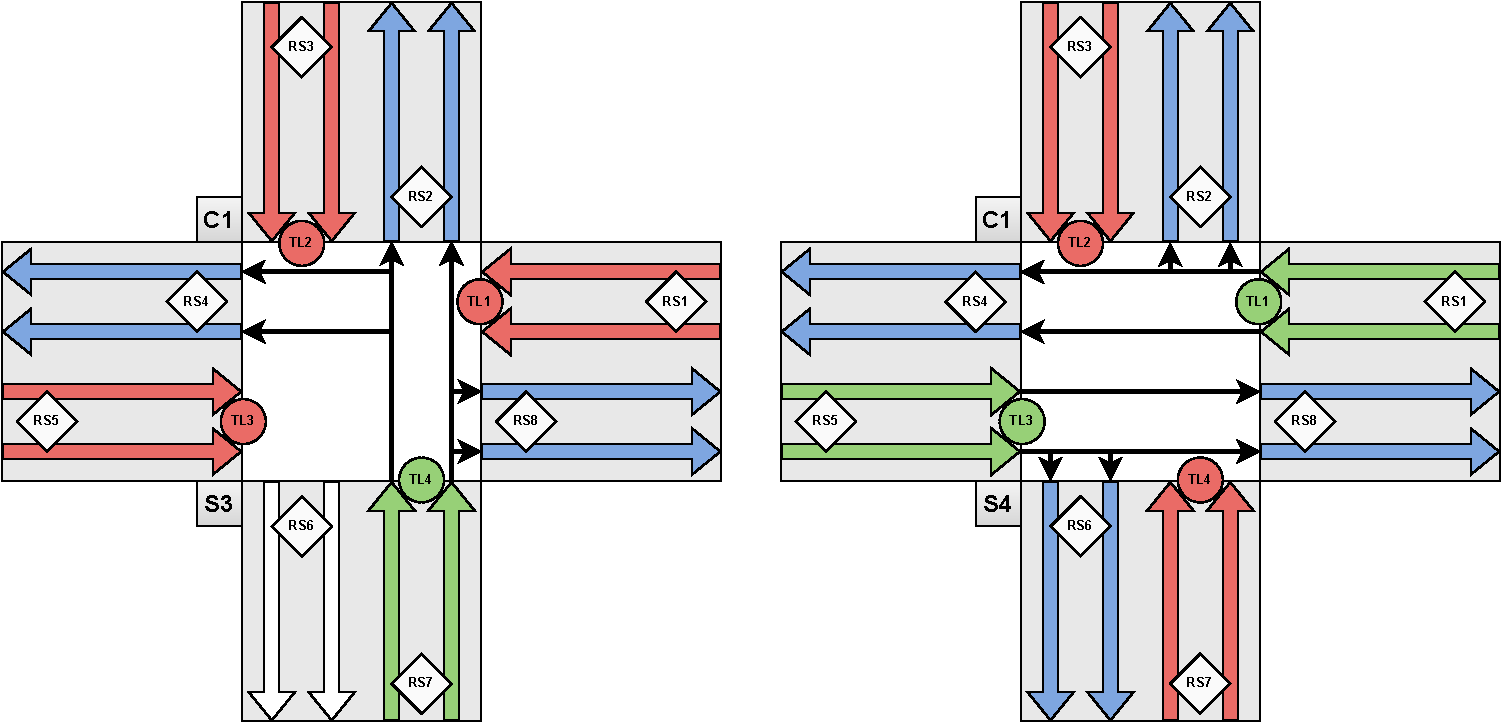
\includegraphics[width=1\linewidth]{text/image/DCruc-CE-Estados3y4.pdf}
    \caption{Cruce estándar en estados 3 y 4}
    \label{fig:cruce_estandar_estados_3y4}
\end{figure}

\newpage
El \textbf{quinto estado}, expuesto en la figura \ref{fig:cruce_estandar_estados_5y6}:
\begin{itemize}
    \item habilita el tránsito de vehículos desde el tramo de calle \textbf{RS1} hasta los tramos de calle \textbf{RS2}, \textbf{RS4} y \textbf{RS6}, es decir, habilita los tramos de cruce \textbf{RS1-RS2}, \textbf{RS1-RS4} y \textbf{RS1-RS6};
    \item y bloquea el tránsito de vehículos desde los tramos de calle \textbf{RS3}, \textbf{RS5} y \textbf{RS7}.
\end{itemize}

El \textbf{sexto estado}, expuesto en la figura \ref{fig:cruce_estandar_estados_5y6}:
\begin{itemize}
    \item habilita el tránsito de vehículos desde el tramo de calle \textbf{RS5} hasta los tramos de calle \textbf{RS2}, \textbf{RS6} y \textbf{RS8}, es decir, habilita los tramos de cruce \textbf{RS5-RS2}, \textbf{RS5-RS6} y \textbf{RS5-RS8};
    \item y bloquea el tránsito de vehículos desde los tramos de calle \textbf{RS1}, \textbf{RS3} y \textbf{RS7}.
\end{itemize}
\begin{figure}[H]
    \centering
    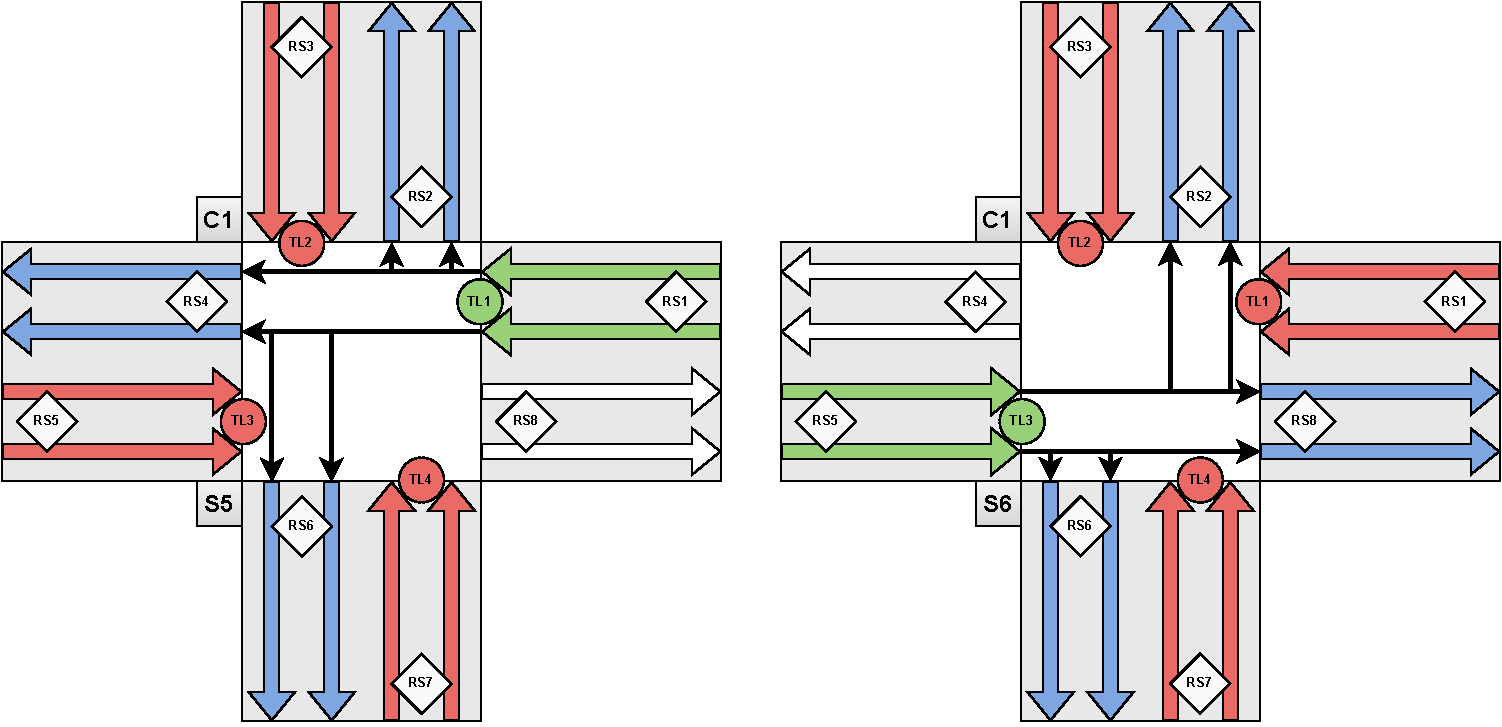
\includegraphics[width=1\linewidth]{text/image/DCruc-CE-Estados5y6.pdf}
    \caption{Cruce estándar en estados 5 y 6}
    \label{fig:cruce_estandar_estados_5y6}
\end{figure}


\newpage
\section{Sociedad de agentes}
    \label{section:sociedad_de_agentes}
El sistema MURAT es una construcción software basada en una arquitectura multiagente. Esto implica que existen uno o más tipos de agentes con roles definidos y propósitos específicos. Asimismo, existen uno o más agentes de cada tipo. Estos agentes, para el cumplimiento de sus objetivos, se encuentran organizados en una sociedad.
\begin{figure}[H]
    \centering
    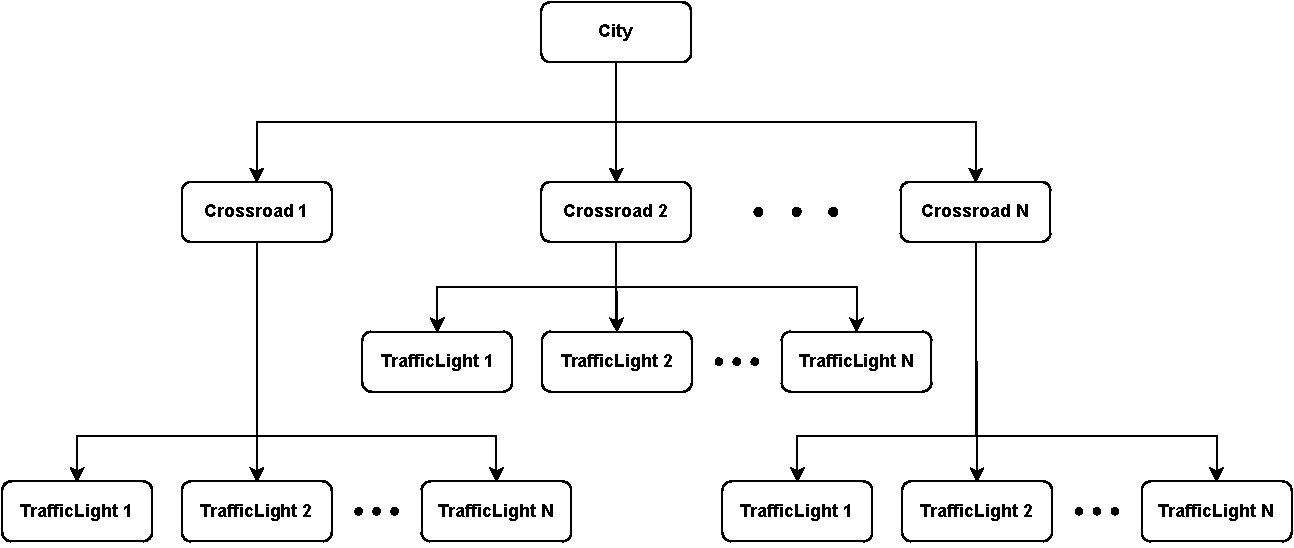
\includegraphics[width=1\linewidth]{text/image/DAgen-Sociedad_de_agentes.pdf}
    \caption{Sociedad de agentes del sistema MURAT}
    \label{fig:sociedad_de_agentes}
\end{figure}
Como se puede observar en la imagen, los agentes están organizados en una sociedad jerárquica. 
%
% ¿Por qué has elegid esta estructura y no otra?
%
\begin{itemize}
    \item \textbf{Ciudad} (\textit{City}): Se encarga de obtener la información del estado de los cruces y generar los informes.
    \item \textbf{Cruce} (\textit{Crossroad}): Se encargan de realizar la simulación, coordinar a los agentes \textit{Semáforo} e informar sobre el estado de la simulación al agente \textit{Ciudad}.
    \item \textbf{Semáforo} (\textit{TrafficLight}): Se encargan de escuchar las órdenes de los agentes \textit{Cruce} y establecer el color de sus luces en función de las mencionadas órdenes.
\end{itemize}

Sin embargo, no todas las relaciones entre agentes son de tipo jerárquico:
\begin{itemize}
    \item Los agentes \textit{Semáforo} obedecen órdenes directas de los agentes \textit{Cruce}. Hasta que un agente \textit{Cruce} no ordene un cambio de estado a un agente \textit{Semáforo} el agente \textit{Semáforo} no cambiará de color. En esta relación se puede observar una fuerte jerarquización, los agentes \textit{Cruce} controlan a los agentes \textit{Semáforo}.
    \item Los agentes \textit{Cruce} colaboran con el agente \textit{Ciudad} enviando los informes sobre el estado de la simulación en cada instante. El agente \textit{Ciudad} informa de que puede continuar la simulación una vez recibidos los informes de todos los agentes \textit{Cruce}. En esta relación se puede observar una estructura en red basada en la colaboración para la consecución de objetivos comunes. No obstante, el agente \textit{Ciudad} ordena a los agentes \textit{Cruce} que finalicen cuando ha terminado la simulación. Esto es una acción de control por parte del agente \textit{Ciudad} sobre el agente \textit{Cruce}; otra vez se puede apreciar una estructura jerárquica.
\end{itemize}

Los agentes tienen acceso a los datos que necesitan para su correcto funcionamiento. Gran parte de la información de carga del modelo del entorno está almacenada en estructuras de datos de la clase \textit{Simulation}. A esta información acceden los agentes a través de determinadas funciones definidas en la propia clase; este conjunto de funciones actuaría como una interfaz, haciendo las veces de una \acrshort{api}. Cuando es necesario, por ejemplo, para los cambios de color de los semáforos o la transferencia de vehículos, se intercambia la información necesaria a través de paso de mensajes.

%%% ------------------------ Agente SEMÁFORO ------------------------ %%%
\subsection{Agente Semáforo (TrafficLight)}
El agente \textit{Semáforo} es el agente más simple de la sociedad. Se encuentra en la posición menos privilegiada de la jerarquía. Opera a merced del único agente \textit{Cruce} que se encarga de él. Sus capacidades son: cambiar su luz de rojo a verde o de verde a rojo; y poner la luz del color que haya ordenado el agente \textit{Cruce}. 

\subsubsection{Estados del agente}
\begin{enumerate}
    \item \textbf{Cargar datos} \footnotesize(LOAD\_DATA)\normalsize: Estado en el que se cargan los datos necesarios para el funcionamiento del agente.
    \begin{itemize}
        \item Se obtienen los datos del cruce al que pertenece.
        \item Se obtienen los datos del tramo de calle que regula.
    \end{itemize}
    Una vez se ha cargado la información, el agente \textit{Semáforo} cambia al siguiente estado.
    \item \textbf{Escuchar al cruce} \footnotesize(LISTEN\_CROSSROAD)\normalsize: Estado en el que se escuchan mensajes para recibir mensajes provenientes del agente \textit{Cruce}. Mientras que el agente se encuentra en este estado permanece en una escucha continua de mensajes. Hay que tener en cuenta que el agente \textit{Semáforo} no sabe por sí mismo si el estado que posee es correcto en relación al resto de sistema, únicamente lo puede saber cuando se lo dice el agente \textit{Cruce}.
    \begin{itemize}
        \item Espera la inicialización por parte del agente \textit{Cruce}.
        \item Espera cualquier solicitud por parte del agente \textit{Cruce}.
            \begin{itemize}
                \item Cambiar de color.
                \item Poner el color en rojo.
                \item Poner el color en verde.
                \item Finalizar.
            \end{itemize}
    \end{itemize}
    \item \textbf{Salir} \footnotesize(EXIT)\normalsize: Estado en el que el agente finaliza su ejecución. Un agente \textit{Semáforo} nunca se podrá apagar si no es por orden del agente superior de la sociedad jerárquica a la que pertenece; siguiendo el flujo del software, a este estado solo se puede llegar tras la orden del agente \textit{Cruce}.
\end{enumerate}

\subsubsection{Diagrama de secuencia del agente}
\begin{figure}[H]
    \centering
    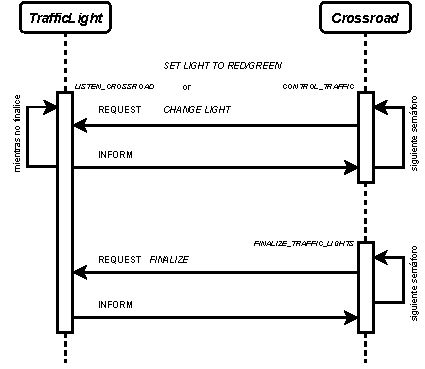
\includegraphics[width=1\linewidth]{text/image/DAgen-DS-TrafficLight.pdf}
    \caption{Diagrama de secuencia del agente \textit{Semáforo}}
    \label{fig:ds_agente_semaforo}
\end{figure}

\subsubsection{Diagrama de clases del agente}
\begin{figure}[H]
    \centering
    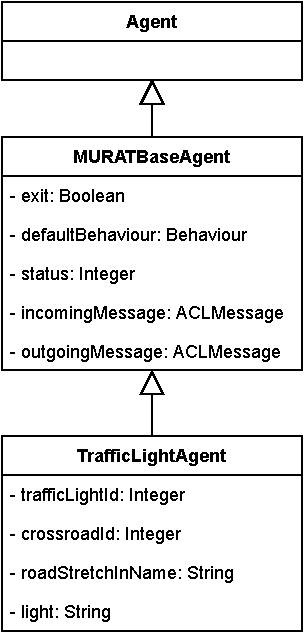
\includegraphics[width=0.35\linewidth]{text/image/DAgen-DC-TrafficLight.pdf}
    \caption{Diagrama de clases del agente \textit{Semáforo}}
    \label{fig:dc_agente_semaforo}
\end{figure}

\subsubsection{Diagrama de actividad del agente}
\begin{figure}[H]
    \centering
    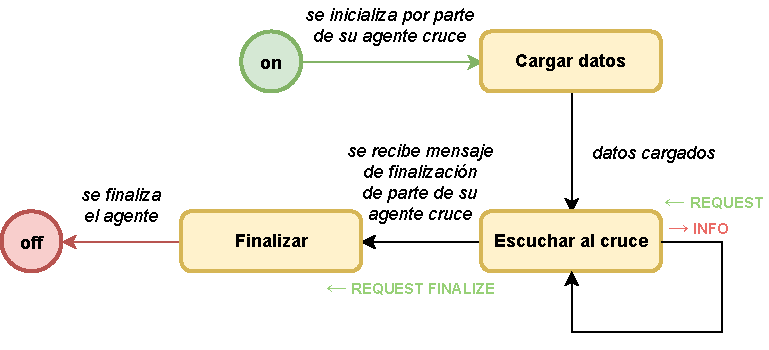
\includegraphics[width=1\linewidth]{text/image/DAgen-DA-TrafficLight.pdf}
    \caption{Diagrama de actividad del agente \textit{Semáforo}}
    \label{fig:da_agente_semaforo}
\end{figure}
%%% --------------------------------------------------------------- %%%

%%% ------------------------ Agente CRUCE ------------------------ %%%
\subsection{Agente Cruce (Crossroad)}
El agente \textit{Cruce} es el agente más complejo de la sociedad. Este agente es el encargado de controlar la simulación y comunicarse con el resto de agentes. Ordena los cambios de luz a los agentes \textit{Semáforo}, informa de su estado al agente \textit{Ciudad} y se comunica con otros agentes \textit{Cruce} para recibir y/o enviar vehículos.

\subsubsection{Estados del agente}
\begin{enumerate}
    \item \textbf{Cargar datos} \footnotesize(LOAD\_DATA)\normalsize: Estado en el que se cargan los datos necesarios para el funcionamiento del agente.
    \begin{itemize}
        \item Se obtienen los datos del nombre de la ciudad.
        \item Se obtienen los datos del modo de entrada del tráfico a la simulación.
        \item Se obtienen los datos de si la política de optimización de tiempos está activa o no.
        \item Se obtienen los datos generales de cada del cruce.
        \item Se obtienen los datos de los estados del cruce.
        \item Se obtienen los datos del estado inicial del cruce.
        \item Se obtienen los datos de los semáforos del cruce.
        \item Se obtienen los datos de los colores de semáforos para cada estado del cruce.
        \item Se obtienen los datos de los tramos de calle conectados al cruce.
        \item Se obtienen los datos de los tramos de cruce.
        \item Se obtienen los datos de los tramos de cruce abiertos por cada semáforo en verde en cada estado.
        \item Se obtienen los datos del tiempo de muestreo.
        \item Se obtienen los datos del tiempo de inicio de la simulación.
        \item Se obtienen los datos de los segundos totales de duración de la simulación.  \item Se inicializan diferentes estructuras de datos.
    \end{itemize}
    Una vez se ha cargado la información, el agente \textit{Cruce} cambia al siguiente estado.
    \item \textbf{Inicializar semáforos} \footnotesize(INITIALIZE\_TRAFFIC\_LIGHTS)\normalsize: Estado en el que el agente inicializa a los agentes \textit{Semáforo}. Se envía un mensaje a cada semáforo para inicializarlo con en color que corresponda en función del estado inicial del cruce.
    \item \textbf{Controlar el tráfico} \footnotesize(CONTROL\_TRAFFIC)\normalsize: Estado en el que el agente realiza todos los procesos relativos a la simulación.
    \begin{itemize}
        \item Almacena el estado estado actual del cruce.
        \item Informa al agente \textit{Ciudad} del estado actual del cruce.
        \item Comprueba si ha finalizado la simulación.
        \item Comprueba si hay que cambiar de estado.
        \item Mueve a los vehículos de un tramo de calle a otro tramo de calle. Hace que los vehículos pasen por el tramo de cruce.
        \begin{itemize}
            \item Mueve los vehículos fuera del sistema de tráfico o a otros cruces.
            \item Recibe vehículos de otros agentes \textit{Cruce}.
            \item Mueve los vehículos haciendo que crucen por un tramo de cruce.
        \end{itemize}
        \item Añade vehículos a la simulación.
        \item Optimiza los tiempos de los estados en función de las condiciones de saturación de los tramos de calle.
        \item Pasa al siguiente instante de la simulación.
    \end{itemize}
    Todos estos pasos son repetidos hasta que finaliza la simulación. En este momento es cuando el agente \textit{Ciudad} ordena a los agentes \textit{Cruce} que pasen al siguiente estado.
    \item \textbf{Finalizar semáforos} \footnotesize(FINALIZE\_TRAFFIC\_LIGHTS)\normalsize: Estado en el que el agente finaliza a los agentes \textit{Semáforo}. Las órdenes de finalización son enviadas a los agentes \textit{Semáforo} una vez ha finalizado la simulación y se han enviado todos los informes de la misma al agente \textit{Ciudad}.
    \item \textbf{Salir} \footnotesize(EXIT)\normalsize: Estado en el que el agente finaliza su ejecución. Un agente \textit{Cruce} nunca se podrá apagar si no es por orden del agente superior de la sociedad jerárquica a la que pertenece; siguiendo el flujo del software, a este estado solo se puede llegar tras la orden del agente \textit{City}.
\end{enumerate}

\newpage
\subsubsection{Diagrama de secuencia del agente}
%
% ¿Qué es esto? ¿PAra qué sirve? Yo sí lo sé XD pero el que lea esto no 
%

\begin{figure}[H]
    \centering
    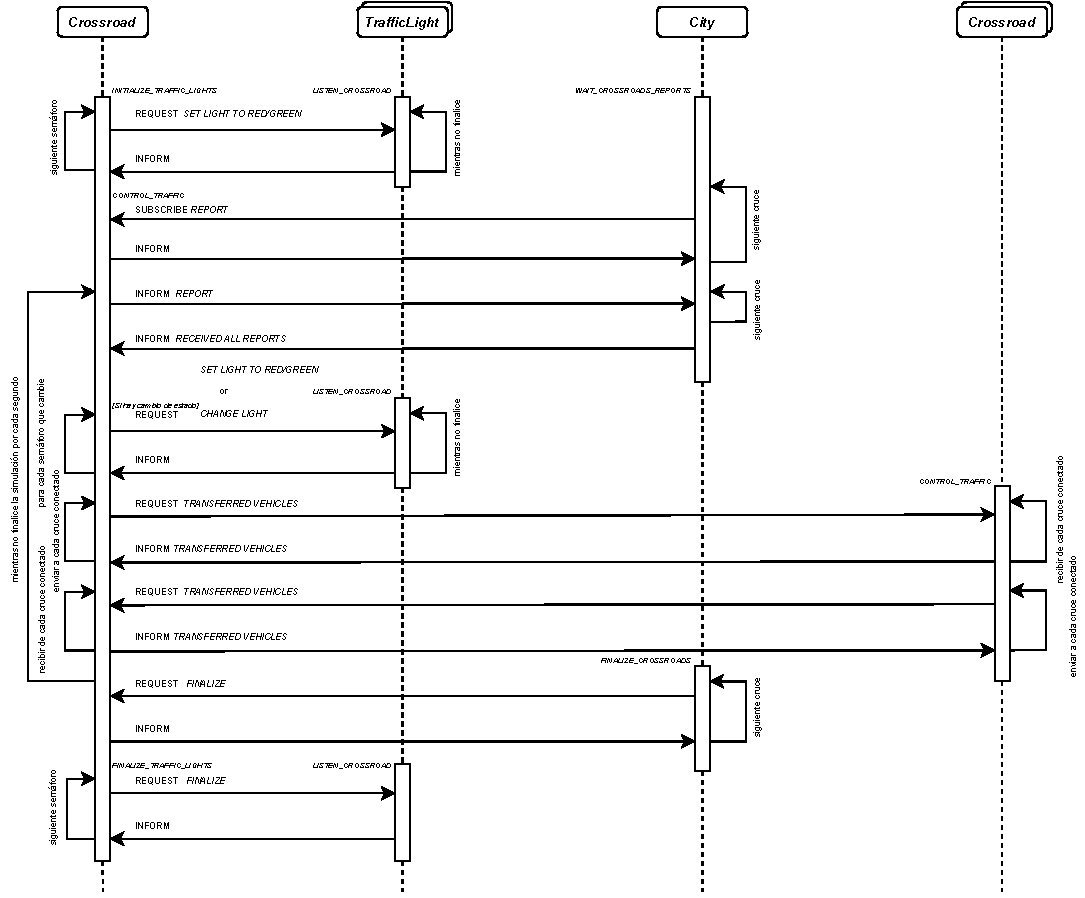
\includegraphics[width=1\linewidth]{text/image/DAgen-DS-Crossroad.pdf}
    \caption{Diagrama de secuencia del agente \textit{Cruce}}
    \label{fig:ds_agente_cruce}
\end{figure}

\newpage
\subsubsection{Diagrama de clases del agente}
\begin{figure}[H]
    \centering
    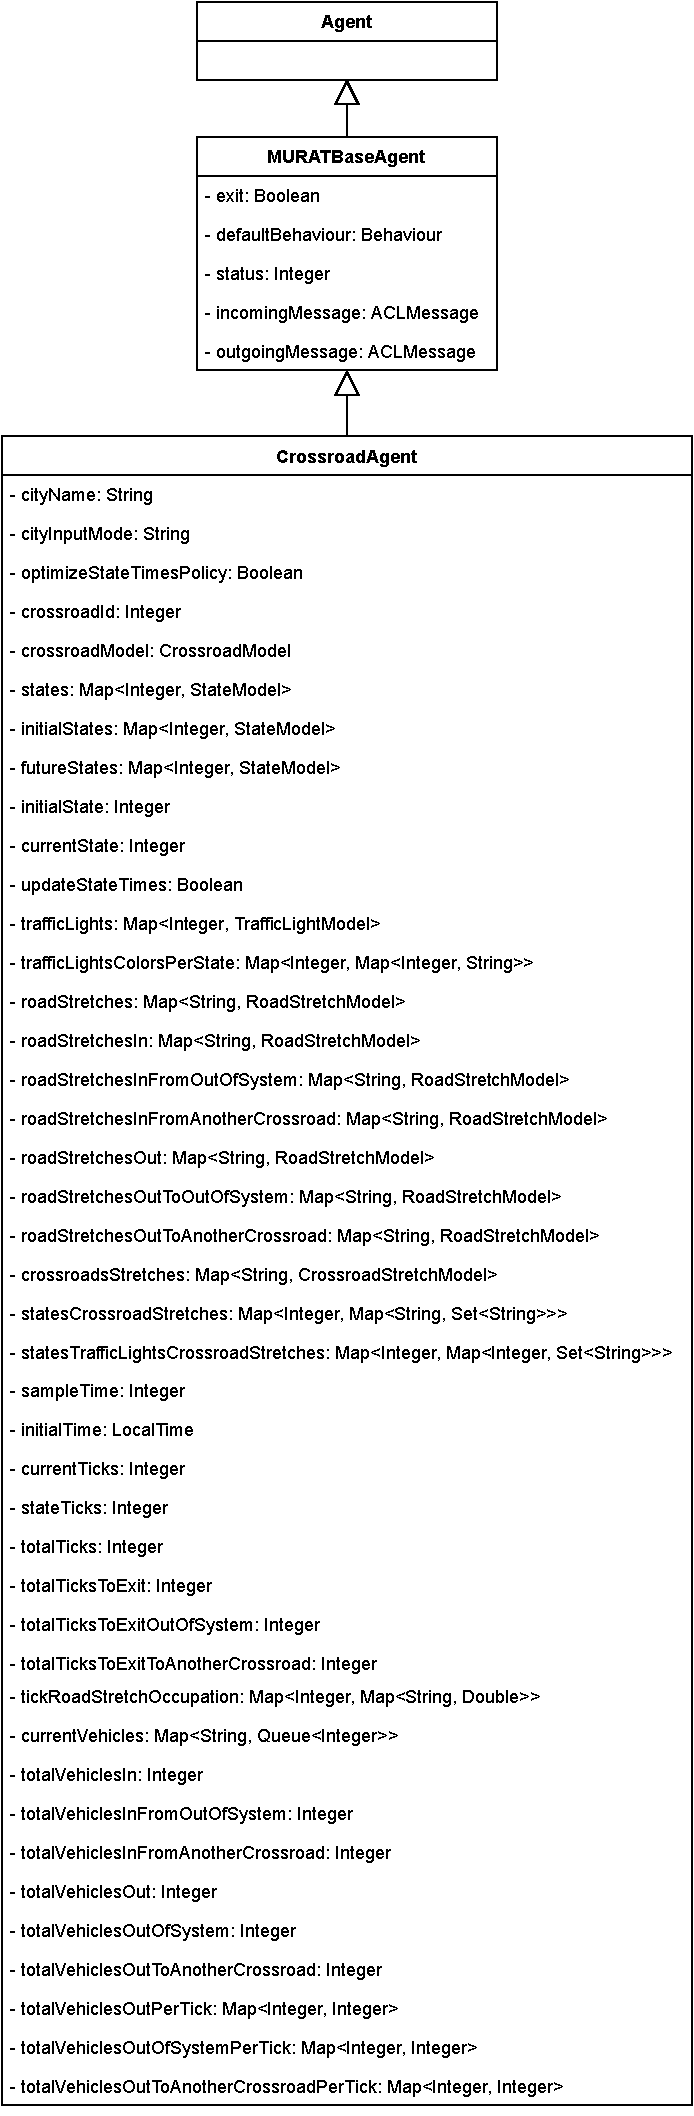
\includegraphics[width=0.50\linewidth]{text/image/DAgen-DC-Crossroad.pdf}
    \caption{Diagrama de clases del agente \textit{Cruce}}
    \label{fig:dc_agente_cruce}
\end{figure}

\newpage
\subsubsection{Diagrama de actividad del agente}
\begin{figure}[H]
    \centering
    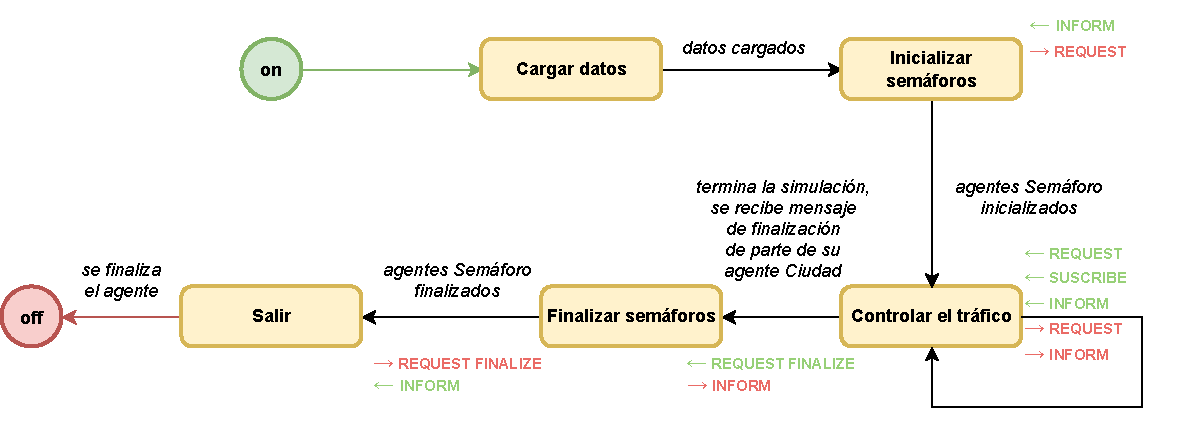
\includegraphics[width=1\linewidth]{text/image/DAgen-DA-Crossroad.pdf}
    \caption{Diagrama de actividad del agente \textit{Cruce}}
    \label{fig:da_agente_cruce}
\end{figure}
%%% --------------------------------------------------------------- %%%

%%% ------------------------ Agente CIUDAD ------------------------ %%%
\subsection{Agente Ciudad (City)}
El agente \textit{Ciudad} es el agente encargado de recibir la información del estado de los agentes \textit{Cruce} en cada instante de la simulación y generar los informes correspondientes. Este agente es único en el sistema. Se comunica con todos y cada uno de los agentes \textit{Cruce}.

\subsubsection{Estados del agente}
\begin{enumerate}
    \item \textbf{Cargar datos} \footnotesize(LOAD\_DATA)\normalsize: Estado en el que se cargan los datos necesarios para el funcionamiento del agente.
    \begin{itemize}
        \item Se obtienen los datos de los cruces de la ciudad.
        \item Se obtienen los datos de los nombres de los cruces de la ciudad.
        \item Se obtienen los datos de los nombres de las calles de la ciudad.
        \item Se obtienen los datos del tiempo de muestreo.
        \item Se obtienen los datos del tiempo de inicio de la simulación.
        \item Se obtienen los datos del los segundos totales de duración de la simulación.
        \item Se inicializan diferentes estructuras de datos.
    \end{itemize}
    Una vez se ha cargado la información, el agente \textit{Ciudad} cambia al siguiente estado.
    \item \textbf{Escuchar informes de los cruces} \footnotesize(WAIT\_CROSSROADS\_REPORTS)\normalsize: Estado en el que se escuchan mensajes provenientes de los agentes \textit{Cruce} con el objetivo de recibir informes del estado local de la simulación en cada cruce. Por cada segundo de la simulación cada agente \textit{Cruce} envía un informe al agente \textit{Ciudad} sobre su estado local en la simulación. El agente \textit{Ciudad} no autoriza a los agentes \textit{Cruce} a que continúen la simulación hasta que no haya recibido todos los informes del instante correspondiente de la simulación.
    \begin{itemize}
        \item Espera mensajes con la performativa \textit{inform} provenientes del agente \textit{Cruce}.
            \begin{itemize}
                \item Actualiza la información del estado de la simulación.
                \item Etiqueta el informe del agente \textit{Cruce} como recibido.
                \item Autoriza a los agentes \textit{Cruce} a continuar la simulación si se han recibido todos los informes para el instante correspondiente.
                \item Comprueba si ha finalizado la simulación.
            \end{itemize}
    \end{itemize}
    \item \textbf{Generar informe de la simulación} \footnotesize(GENERATE\_SIMULATION\_ \newline REPORT)\normalsize: Estado en el que el agente genera un informe de la simulación en formato \textit{\acrshort{csv}}. Para poder crear el informe se deben haber recibido previamente los informes de todos los cruces para cada instante de la simulación.
    \item \textbf{Finalizar cruces} \footnotesize(FINALIZE\_CROSSROADS)\normalsize: Estado en el que el agente finaliza a los agentes \textit{Cruce}. Una vez se han recibido todos los informes de la simulación y se ha generado el informe de la misma se puede determinar que la simulación ha finalizado y, por tanto, que los agentes \textit{Cruce} deben ser apagados.
    \item \textbf{Salir} \footnotesize(EXIT)\normalsize: Estado en el que el agente finaliza su ejecución. El agente \textit{Ciudad} es el único agente en apagarse por decisión propia; siguiendo el flujo del software, a este estado solo se puede llegar tras haber recibido todos los informes de simulación por parte de los agentes \textit{Cruce}, haber generado el informe de la simulación y haber finalizado a los agentes \textit{Cruce}.
\end{enumerate}

\subsubsection{Diagrama de secuencia del agente}
\begin{figure}[H]
    \centering
    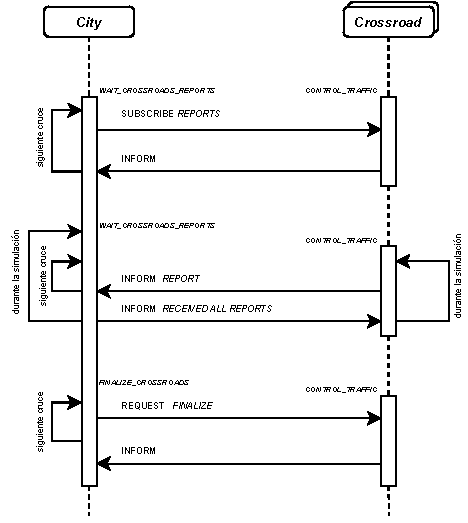
\includegraphics[width=0.85\linewidth]{text/image/DAgen-DS-City.pdf}
    \caption{Diagrama de secuencia del agente \textit{Ciudad}}
    \label{fig:ds_agente_ciudad}
\end{figure}

\newpage
\subsubsection{Diagrama de clases del agente}
\begin{figure}[H]
    \centering
    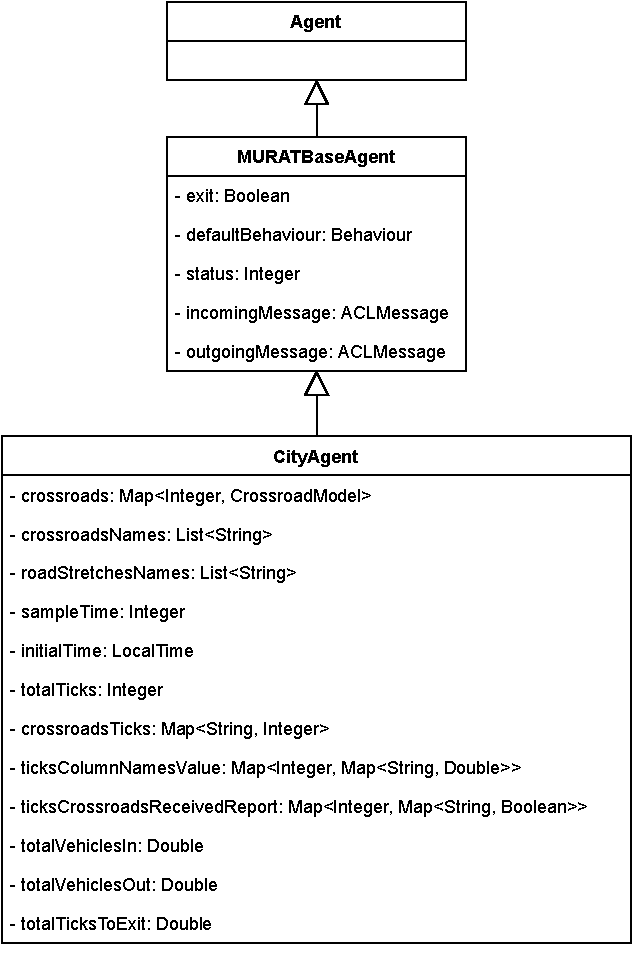
\includegraphics[width=0.60\linewidth]{text/image/DAgen-DC-City.pdf}
    \caption{Diagrama de clases del agente \textit{Ciudad}}
    \label{fig:dc_agente_ciudad}
\end{figure}

\subsubsection{Diagrama de actividad del agente}
\begin{figure}[H]
    \centering
    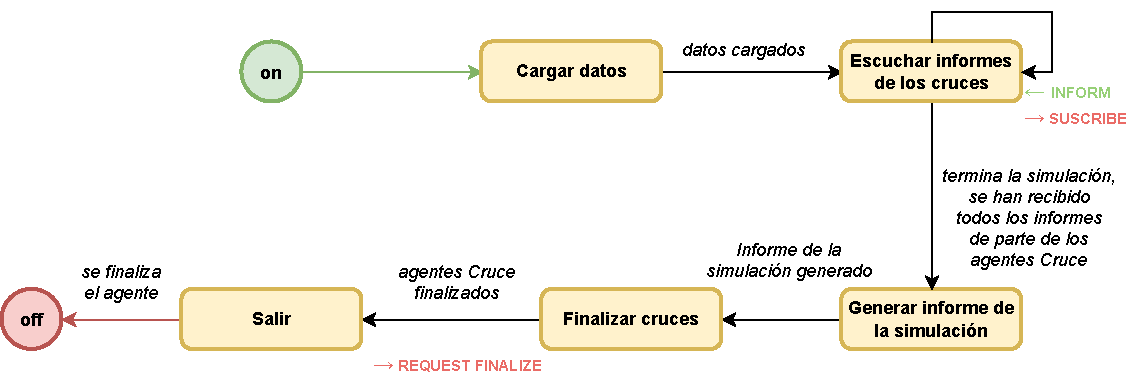
\includegraphics[width=1\linewidth]{text/image/DAgen-DA-City.pdf}
    \caption{Diagrama de actividad del agente \textit{Ciudad}}
    \label{fig:da_agente_ciudad}
\end{figure}
%%% --------------------------------------------------------------- %%%

\subsection{Diagrama de clases de los agentes}
\begin{figure}[H]
    \centering
    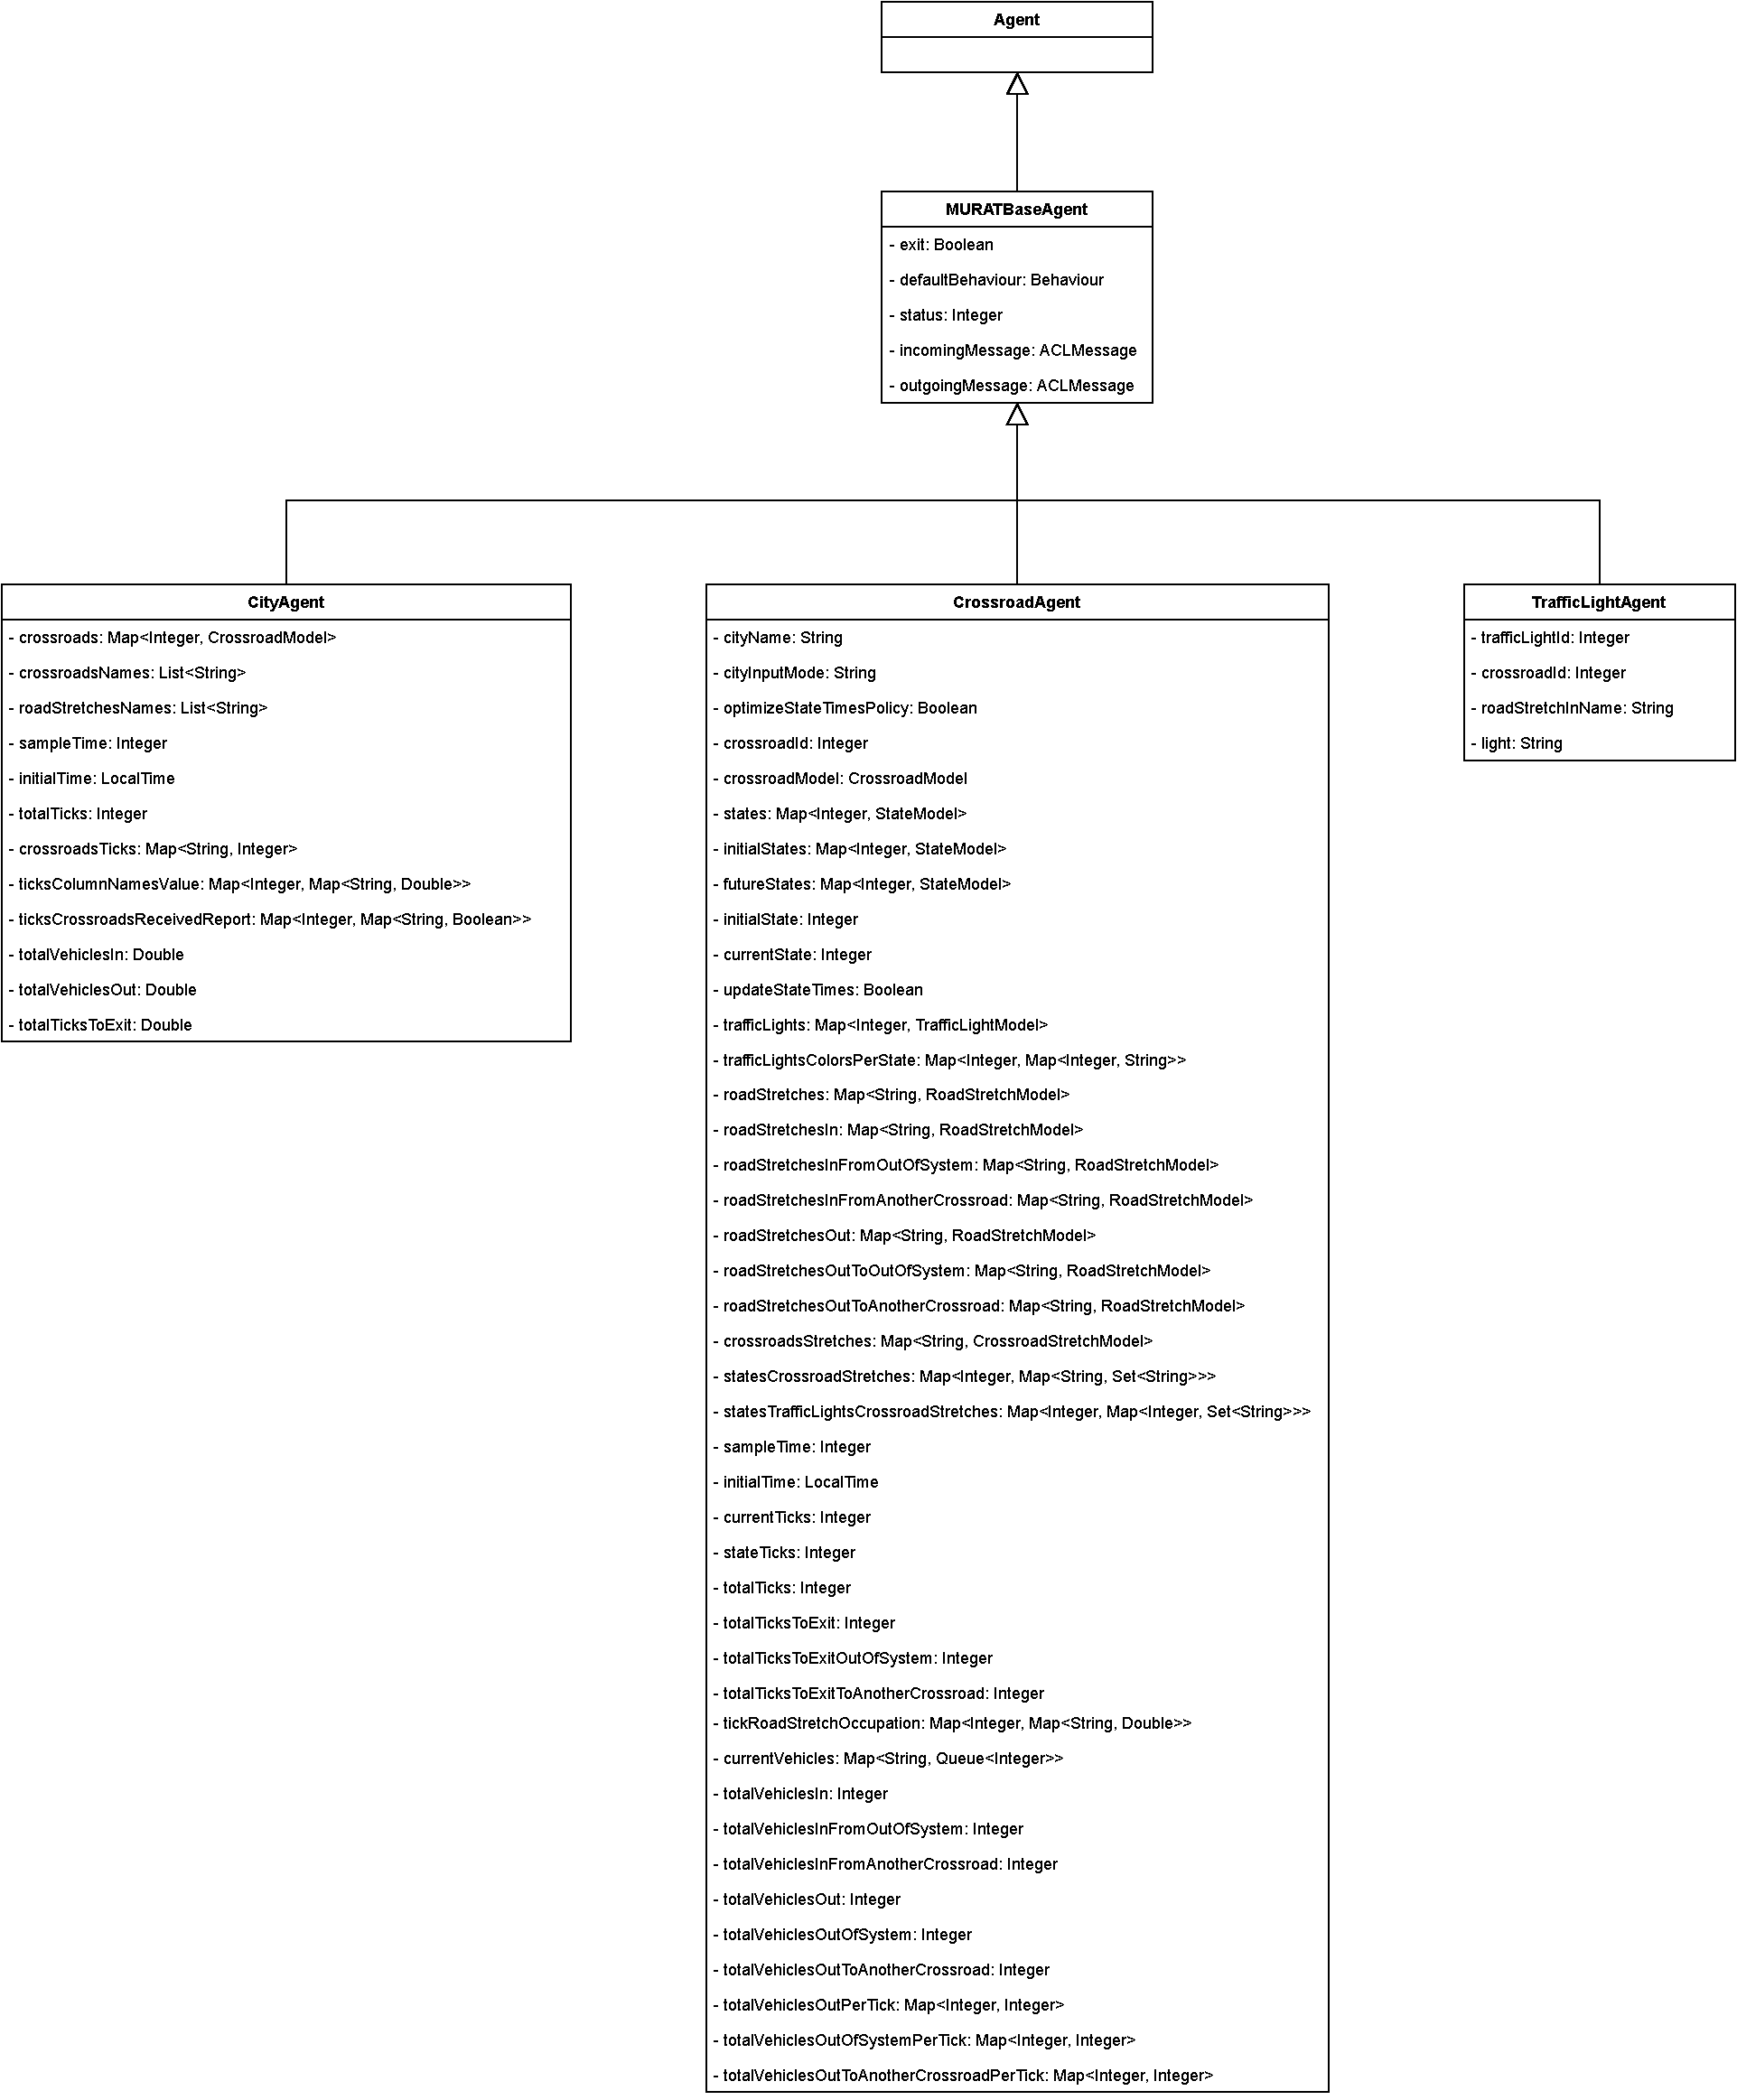
\includegraphics[width=1\linewidth]{text/image/DAgen-DC.pdf}
    \caption{Diagrama de clases de los agentes}
    \label{fig:dc_agentes}
\end{figure}

\newpage
\section{Modelo de datos de representación de la realidad}
En esta sección se expone el modelo de datos diseñado con el objetivo de realizar una representación precisa de la información del mundo real. Dicho modelo de datos es el nexo de unión entre las diferentes topologías de ciudades reales y sus correspondientes representaciones en el sistema MURAT. Este modelo de datos ha sido planteado de tal manera que permita representar desde una hasta varias ciudades, las cuales pueden poseer diferente complejidad.

\newpage
\subsection{Diagrama del modelo entidad-relación (E/R)}
\begin{figure}[H]
    \centering
    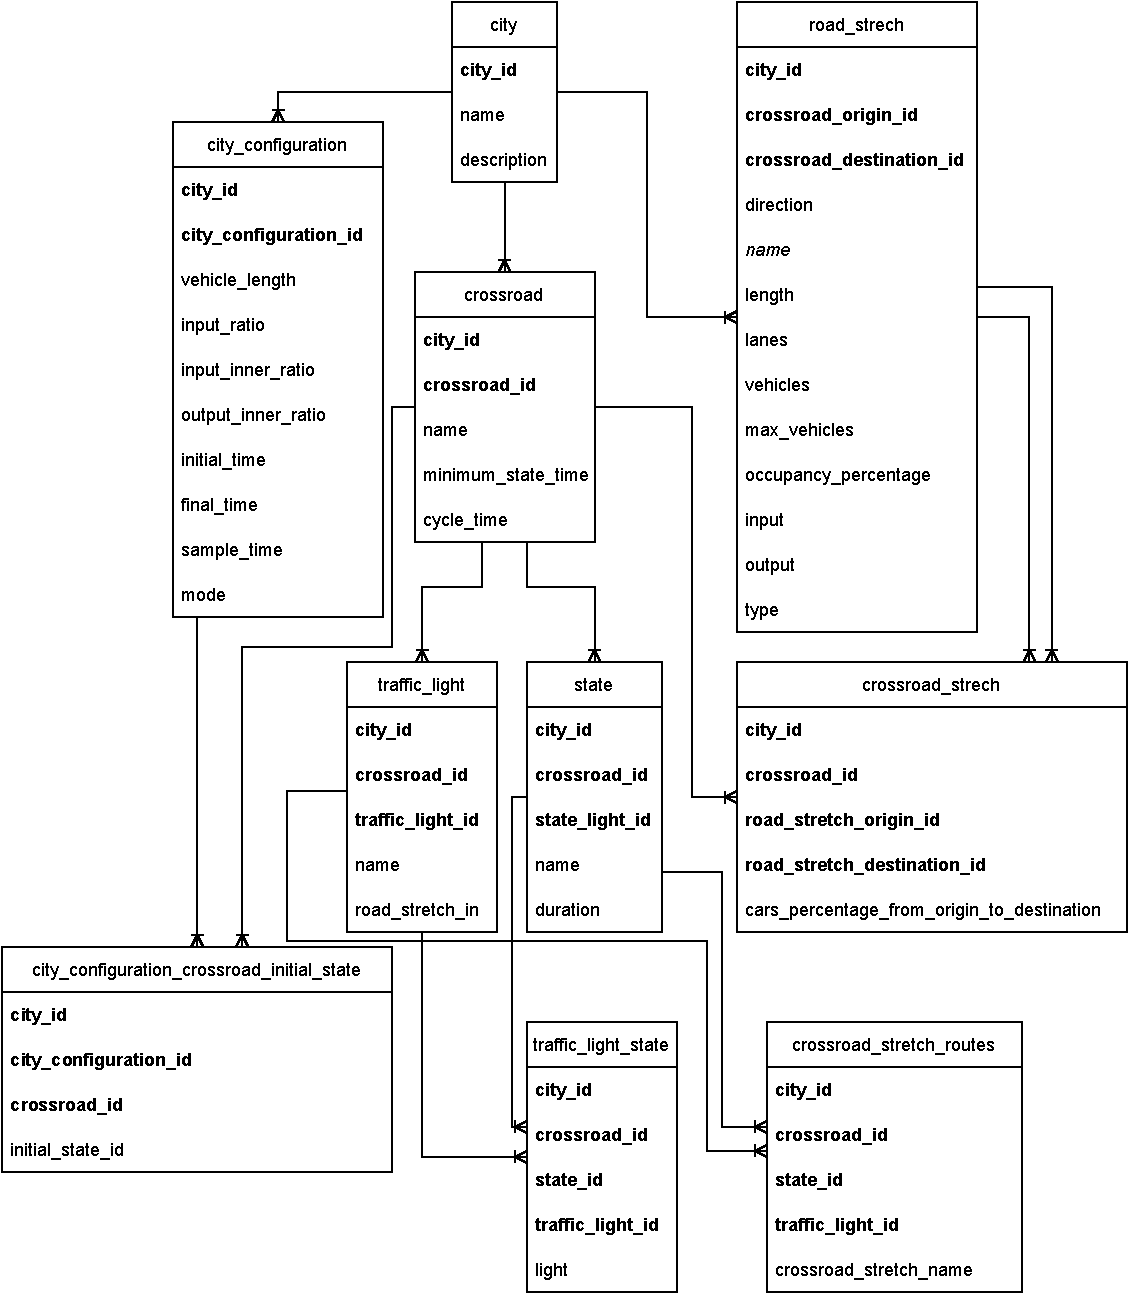
\includegraphics[width=1\linewidth]{text/image/DE_R.pdf}
    \caption{Diagrama E/R del modelo de datos propuesto}
    \label{fig:de_r}
\end{figure}

\newpage
\subsection{Representación en tablas}
La representación se realiza a través de un modelo basado en tablas, con un total de diez tablas:

\subsubsection{Tabla - Ciudad (\textit{city})}
En esta tabla se almacena la información básica, nombre y descripción, de las diferentes ciudades que están representadas y disponibles para ser simuladas en el sistema MURAT. \\\\
Atributos:
\begin{itemize}
    \item \textbf{Id de la ciudad} (\textit{city\_id}): identificador de la ciudad.
    \item \textbf{Nombre} (\textit{name}): nombre de la ciudad.
    \item \textbf{Descripción} (\textit{description}): descripción de la ciudad. Información extra de la ciudad.
\end{itemize}
\textbf{Clave primaria}: \{\textit{city\_id}\}. \\

\subsubsection{Tabla - Configuración de ciudad (\textit{city\_configuration})}
En esta tabla se almacena la información relativa a las diferentes configuraciones disponibles para cada ciudad. El sistema MURAT puede simular diferentes ciudades. Cada una de estas ciudades puede tener, a su vez, diferentes tipos de configuración. Por ejemplo, si para la misma ciudad se quieren realizar varias simulaciones que empiecen y/o terminen a horas diferentes se pueden crear y seleccionar diferentes tipos de configuración. O bien, si se desea que haya diferentes flujos de entrada de vehículos al sistema, también se pueden crear y elegir otras configuraciones.\\\\
Atributos:
\begin{itemize}
    \item \textbf{Id de la ciudad} (\textit{city\_id}): identificador de la ciudad.
    \item \textbf{Id de la configuración} (\textit{city\_configuration\_id}): identificador de la configuración.
    \item \textbf{Longitud de vehículo} (\textit{vehicle\_length}): longitud que mide un vehículo.
    \item \textbf{Ratio de entrada} (\textit{input\_ratio}): relación de entrada de tráfico al sistema. Cantidad de vehículos que se añaden a la simulación de tráfico por vía de tramo de calle y segundo.
    \item \textbf{Ratio interno de entrada} (\textit{input\_inner\_ratio}): relación de entrada de tráfico interna del sistema, es decir, desde unos cruces a otros cruces. Cantidad de vehículos que se mueven en un tramo de calle interno desde un cruce hasta otro cruce, es decir, número de vehículos que entran a los tramos de calle interiores (\textit{RoadStretchIn}) por vía y segundo.
    \item \textbf{Ratio interno de salida} (\textit{output\_inner\_ratio}): relación de salida de tráfico interna del sistema, es decir, o desde unos cruces hasta otros cruces o desde unos cruces hacia fuera del sistema. Cantidad de vehículos que salen, bien de tramos de calle entre cruces, bien de la simulación por vía y segundo.
    \item \textbf{Hora de inicio} (\textit{initial\_time}): hora de inicio de la simulación.
    \item \textbf{Hora de fin} (\textit{final\_time}): hora de fin de la simulación.
    \item \textbf{Tiempo de muestreo} (\textit{sample\_time}): tiempo de muestreo de la simulación. Cantidad de tiempo que pasa desde que se toma una muestra del estado de la simulación hasta que se toma la siguiente.
    \item \textbf{Modo} (\textit{mode}): modo en el que los vehículos se van añadiendo al sistema. En el sistema se contemplan tres valores:
    \begin{itemize}
        \item \textit{Lineal} (\textbf{LINEAR}): durante toda la simulación entra al sistema de tráfico la misma cantidad de vehículos.
        \item \textit{Pico único} (\textbf{SINGLE PEAK}): durante toda la simulación entra al sistema de tráfico la misma cantidad de vehículos a excepción de en un intervalo pico determinado, donde entra una cantidad mucho mayor. Esto, en la realidad se asemejaría, por ejemplo, al intervalo de 08:00 a 09:00, donde existe mayor afluencia de tráfico.
        \item \textit{Pico doble} (\textbf{DOUBLE PEAK}): durante toda la simulación entra al sistema de tráfico la misma cantidad de vehículos a excepción de en dos intervalos pico determinados, donde entran unas cantidades mucho mayores. Esto, en la realidad se asemejaría, por ejemplo, a los intervalos de 08:00 a 09:00 y de 19:00 a 20:00, donde existe mayor afluencia de tráfico.
    \end{itemize}
\end{itemize}
\textbf{Clave primaria}: \{\textit{city\_id}, \textit{city\_configuration\_id}\}. \\
\textbf{Clave foránea}: \{\textit{city\_id}\} de (\textit{city.city\_id}).

\subsubsection{Tabla - Estado inicial de cruces por configuración\\ (\textit{city\_configuration\_crossroad\_initial\_state})}
En esta tabla se almacena la información de los estados iniciales de cada cruce al inicio de la simulación de tráfico para cada configuración de cada ciudad. Ya se ha explicado que para cada ciudad pueden existir diferentes configuraciones. Cada una de estas configuraciones también define en qué estado está cada cruce al inicio de la simulación. Esta tabla se encarga de almacenar esa información. \\\\
Atributos:
\begin{itemize}
    \item \textbf{Id de la ciudad} (\textit{city\_id}): identificador de la ciudad.
    \item \textbf{Id de la configuración} (\textit{city\_configuration\_id}): identificador de la configuración.
    \item \textbf{Id del cruce} (\textit{crossroad\_id}): identificador del cruce.
    \item \textbf{Id del estado inicial} (\textit{initial\_state\_id}): identificador del estado inicial.
\end{itemize}
\textbf{Clave primaria}: \{\{\textit{city\_id}, \textit{city\_configuration\_id}\}, \textit{crossroad\_id}\}. \\
\textbf{Claves foráneas}: Simples ya añadidas, \{\textit{city\_id}, \textit{city\_configuration\_id}\} \newline de (\textit{city\_configuration}) y \{\textit{crossroad\_id}\} de (\textit{crossroad.crossroad\_id}).

\subsubsection{Tabla - Cruce (\textit{crossroad})}
En esta tabla se almacena la información básica de los diferentes cruces de cada ciudad, los cuales están representados y disponibles para formar parte de una simulación del sistema MURAT. \\\\
Atributos:
\begin{itemize}
    \item \textbf{Id de la ciudad} (\textit{city\_id}): identificador de la ciudad.
    \item \textbf{Id del cruce} (\textit{crossroad\_id}): identificador del cruce.
    \item \textbf{Nombre} (\textit{name}): nombre del cruce.
    \item \textbf{Tiempo mínimo de estado} (\textit{minimum\_state\_time}): tiempo mínimo que debe durar cada uno de los estados de un cruce.
    \item \textbf{Tiempo de ciclo de estados} (\textit{cycle\_time}): tiempo que dura el paso entre todos los estados de un cruce, es decir, desde que un cruce inicia en un estado hasta que vuelve a ese mismo estado habiendo pasado por todos los demás.
\end{itemize}
\textbf{Clave primaria}: \{\textit{city\_id}, \textit{crossroad\_id}\}. \\
\textbf{Clave foránea}: \{\textit{city\_id}\} de (\textit{city.city\_id}).

\subsubsection{Tabla - Semáforo (\textit{traffic\_light})}
En esta tabla se almacena la información básica de los diferentes semáforos que hay en cada uno de los cruces de cada ciudad. Una de la simplificaciones del sistema MURAT es que los semáforos regulan únicamente la entrada de vehículos a un cruce, no la salida, por ello, cada semáforo tiene asociado un tramo de calle de entrada. \\\\
Atributos:
\begin{itemize}
    \item \textbf{Id de la ciudad} (\textit{city\_id}): identificador de la ciudad.
    \item \textbf{Id del cruce} (\textit{crossroad\_id}): identificador del cruce.
    \item \textbf{Id del semáforo} (\textit{traffic\_light\_id}): identificador del semáforo.
    \item \textbf{Nombre} (\textit{name}): nombre del semáforo.
    \item \textbf{Tramo de calle de entrada} (\textit{road\_stretch\_in}): tramo de calle de entrada al cruce regulado por el semáforo.
\end{itemize}
\textbf{Clave primaria}: \{\{\textit{city\_id}, \textit{crossroad\_id}\}, \textit{traffic\_light\_id}\}. \\
\textbf{Claves foráneas}: Simples ya añadidas, \{\textit{city\_id}, \textit{crossroad\_id}\} de (\textit{crossroad}) y \{\textit{road\_stretch\_in}\} de (\textit{road\_stretch.name}).

\subsubsection{Tabla - Estado (\textit{state})}
En esta tabla se almacena la información relativa a los diferentes estados en los que puede estar cada uno de los cruces de cada ciudad. En función del color en el que se encuentren los semáforos de un cruce, el cruce podría estar en un estado u otro. \\\\
Atributos:
\begin{itemize}
    \item \textbf{Id de la ciudad} (\textit{city\_id}): identificador de la ciudad.
    \item \textbf{Id del cruce} (\textit{crossroad\_id}): identificador del cruce.
    \item \textbf{Id del estado} (\textit{state\_id}): identificador del estado.
    \item \textbf{Nombre} (\textit{name}): nombre del estado.
    \item \textbf{Duración} (\textit{duration}): tiempo que dura el estado. El cruce permanece en un estado durante el tiempo que comprende la duración del mismo. Esta duración no puede ni ser inferior al tiempo mínimo de estado (\textit{minimum\_state\_time}) que define el cruce, ni exceder sumado a la duración del resto de estados el tiempo de ciclo de estados (\textit{cycle\_time}) que, también, define el cruce. 
\end{itemize}
\textbf{Clave primaria}: \{\{\textit{city\_id}, \textit{crossroad\_id}\}, {state\_id}\}. \\
\textbf{Claves foráneas}: Simples ya añadidas y \{\textit{city\_id}, \textit{crossroad\_id}\} de (\textit{crossroad}).

\subsubsection{Tabla - Luz de semáforos por estado (\textit{traffic\_light\_state})}
En esta tabla se almacena la información relativa al color de los semáforos para los diferentes estados posibles en los que puede estar cada uno de los cruces de cada ciudad. Como anteriormente se ha descrito, los estados de los cruces están definidos en función del color de los semáforos. Esta tabla es la que asocia cada estado con el color de cada uno de los semáforos. \\\\
Atributos:
\begin{itemize}
    \item \textbf{Id de la ciudad} (\textit{city\_id}): identificador de la ciudad.
    \item \textbf{Id del cruce} (\textit{crossroad\_id}): identificador del cruce.
    \item \textbf{Id del estado} (\textit{state\_id}): identificador del estado.
    \item \textbf{Id del semáforo} (\textit{traffic\_light\_id}): identificador del semáforo.
    \item \textbf{Luz del semáforo} (\textit{light}): color de la luz del semáforo.
\end{itemize}
\textbf{Clave primaria}: \{\{\textit{city\_id}, \textit{crossroad\_id}\}, \textit{state\_id}, \textit{traffic\_light\_id}\}. \\
\textbf{Claves foráneas}: Simples ya añadidas, \{\{\textit{city\_id}, \textit{crossroad\_id}\}, \textit{state\_id}\} de (\textit{state}) y \{\{\textit{city\_id}, \textit{crossroad\_id}\}, \textit{traffic\_light\_id}\} de (\textit{traffic\_light}).

\subsubsection{Tabla - Tramo de calle (\textit{road\_stretch})}
En esta tabla se almacena la información de los tramos de calle de cada ciudad. Cada calle real puede estar constituida por diferentes tramos de calle, que son cada uno de los carriles o conjunto de carriles que van desde un origen diferente hasta un destino igual o diferente y viceversa. \\\\
Atributos:
\begin{itemize}
    \item \textbf{Id de la ciudad} (\textit{city\_id}): identificador de la ciudad.
    \item \textbf{Id del cruce de origen} (\textit{crossroad\_origin\_id}): identificador del cruce de origen.
    \item \textbf{Id del cruce de destino} (\textit{crossroad\_destination\_id}): identificador del cruce de destino.
    \item \textbf{Dirección} (\textit{direction}): dirección desde el cruce de origen hasta el cruce de destino expresada como dirección cardinal: N, NE, E, SE, S, SW, W o NW.
    \item \textbf{Nombre} (\textit{name}): nombre del tramo de calle.
    \item \textbf{Longitud} (\textit{length}): longitud del tramo de calle expresada en metros.
    \item \textbf{Carriles} (\textit{lanes}): número de carriles del tramo de calle.
    \item \textbf{Vehículos} (\textit{vehicles}): número de vehículos que hay en el tramo de calle.
\end{itemize}
Atributos calculados:
\begin{itemize}
    \item \textbf{Vehículos máximos} (\textit{max\_vehicles}): número máximo de vehículos que puede albergar un tramo de calle. Se calcula en base a tras atributos la longitud del tramo de calle, el número de carriles y la longitud por vehículo. Se multiplica la longitud del tramo por el número de carriles y se divide entre la longitud de vehículo.
    \item \textbf{Porcentaje de ocupación} (\textit{occupancy\_percentage}): porcentaje de ocupación del tramo de calle. Es la relación existente entre el número de vehículos que hay en el tramo de calle y el máximo de vehículos que caben en el mismo. Se calcula dividiendo el número de vehículos entre el número máximo de vehículos y multiplicando por cien.
    \item \textbf{Entrada de vehículos} (\textit{input}): cantidad de vehículos que pueden entrar al tramo de calle por segundo. Se calcula en función de su tipo, si es, o bien raíz (ratio de entrada), o bien cualquier otro, interno u hoja (ratio interno de entrada), multiplicando el ratio correspondiente por el número de carriles del tramo de calle.
    \item \textbf{Salida de vehículos} (\textit{output}): cantidad de vehículos que pueden salir de tramo de calle por segundo. Se calcula multiplicando el ratio interno de salida por el número de carriles del tramo de calle.
    \item \textbf{Tipo} (\textit{type}): tipo de tramo de calles. Se identifican los tres siguientes tipos de tramos de calle en función de los valores de los atributos cruce de origen y cruce de destino.
    \begin{itemize}
        \item Si \textbf{no} existe el \textbf{cruce de origen} y existe el \textbf{cruce de destino} se trata de un tramo de calle raíz (\textbf{ROOT}), es decir, un tramo de calle por el que entran vehículos al sistema.
        \item Si existe el \textbf{cruce de origen} y \textbf{no} existe el \textbf{cruce destino} se trata de un tramo de calle hoja (\textbf{LEAF}), es decir, un tramo de calle por el que salen vehículos del sistema.
        \item Si existe el \textbf{cruce de origen} y existe el \textbf{cruce destino} se trata de un tramo de calle interno (\textbf{INNER}), es decir, un tramo de calle por el los vehículos pasan de un cruce a otro.
    \end{itemize}
\end{itemize}
\textbf{Clave primaria}: \{\textit{city\_id}, \{\textit{crossroad\_origin\_id}, \textit{crossroad\_destionation\_id}\}. \\
\textbf{Claves foráneas}: Simples ya añadidas, \{\textit{crossroad\_origin\_id}\} de (\textit{crossroad\_id}) y \{\textit{crossroad\_destination\_id}\} de (\textit{crossroad\_id}).

\subsubsection{Tabla - Tramo de cruce (\textit{crossroad\_stretch})}
En esta tabla se almacena la información de los tramos de cruce de cada uno de los cruces de cada ciudad. Los vehículos, a través del cruce, tienen que ir desde un tramo de calle hasta otro tramo de calle. Esta ruta es a lo que se le llama tramo de cruce. Esta tabla se asemeja a un router que para cada tramo de calle de origen enruta los vehículos a uno o varios tramos de calle de destino. \\\\
Atributos:
\begin{itemize}
    \item \textbf{Id de la ciudad} (\textit{city\_id}): identificador de la ciudad.
    \item \textbf{Id del cruce} (\textit{crossroad\_id}): identificador del cruce.
    \item \textbf{Nombre del tramo de calle de origen} (\textit{road\_strech\_origin\_name}): tramo de calle de origen del vehículo.
    \item \textbf{Nombre del tramo de calle de destino} (\textit{road\_strech\_destination\_name}): tramo de calle de destino del vehículo.
    \item \textbf{Nombre} (\textit{name}): nombre del tramo de cruce. Está formado por la concatenación del nombre del tramo de calle de origen, el separador <<->> y el nombre del tramo de calle de destino.
    \item \textbf{Porcentaje de coches que van de origen a destino}\\ (\textit{cars\_percentage\_from\_origin\_to\_destination}): porcentaje de vehículos interesados en ir desde el tramo de calle de origen hasta el tramo de calle de destino. Desde un tramo de calle de origen se puede ir hacia uno o varios diferentes tramos de calle destino. Cada uno de estos tramos de cruce tendrá un porcentaje de vehículos interesados. La suma de los porcentajes de vehículos cuyos tramos de cruce tienen el mismo origen deben sumar 100\%. Es como decir qué porcentaje de vehículos están interesados en ir desde un origen hasta cada uno de sus destinos. Si desde un origen solo se puede ir hasta un destino, el porcentaje de vehículos interesados es del 100\%. Si desde un origen se pueden ir hacia dos destinos: el primero de ellos una calle principal, muy grande; y el segundo de ellos una calle secundaria, más pequeña; sería una situación racional que el 85\% estuvieran interesados en ir hacia el primer destino y el 15\% restante hacia el segundo destino. 
\end{itemize}
\textbf{Clave primaria}: \{\{\textit{city\_id}, \textit{crossroad\_id}\}, \textit{road\_stretch\_origin\_name}, \newline \textit{road\_stretch\_destination\_name}\}. \\
\textbf{Claves foráneas}: Simples ya añadidas, \{\textit{city\_id}, \textit{crossroad\_id}\} de (\textit{crossroad}), \{\textit{road\_stretch\_origin\_name}\} de (\textit{road\_stretch.road\_stretch\_name}) \newline y \{\textit{road\_stretch\_destination\_name}\} de (\textit{road\_stretch.road\_stretch\_name}).

\subsubsection{Tabla - Rutas de tramos de cruce (\textit{crossroad\_stretch\_routes})}
En esta tabla se almacena la información de los tramos de cruce que habilita cada uno de los semáforos en verde para cada estado de cada uno de los cruces de cada ciudad. Que un semáforo esté en verde significa que los vehículos puedan pasar desde un tramo de calle origen hasta uno o varios tramos de calle destino. Esta tabla es la encargada de almacenar esa información. \\\\
Atributos:
\begin{itemize}
    \item \textbf{Id de la ciudad} (\textit{city\_id}): identificador de la ciudad.
    \item \textbf{Id del cruce} (\textit{crossroad\_id}): identificador del cruce.
    \item \textbf{Id del estado} (\textit{state\_id}): identificador del estado.
    \item \textbf{Id del semáforo} (\textit{traffic\_light\_id}): identificador del semáforo.
    \item \textbf{Nombre del tramo de cruce} (\textit{crossroad\_stretch\_name}): nombre del tramo de cruce. Está formado por la concatenación del nombre del tramo de calle de origen, el separador <<->> y el nombre del tramo de calle de destino.
\end{itemize}
\textbf{Clave primaria}: \{\{\textit{city\_id}, \textit{crossroad\_id}\}, \textit{state\_id}, \textit{traffic\_light\_id}\}. \\
\textbf{Claves foráneas}: Simples ya añadidas, \{\{\textit{city\_id}, \textit{crossroad\_id}\}, \textit{state\_id}\} de (\textit{state}), \{\{\textit{city\_id}, \textit{crossroad\_id}\}, \textit{traffic\_light\_id}\} de (\textit{traffic\_light}) y \newline \{\textit{crossroad\_stretch\_name}\} de (\textit{crossroad\_stretch.name}).

\subsection{Representación en \acrshort{json}}
Finalmente, se ha decidido almacenar la información de los escenarios en un objeto de tipo \acrshort{json} basado en las tablas anteriormente descritas. 

\subsubsection{Análisis del almacenamiento del escenario correspondiente al cruce simple en un objeto de tipo JSON}
En primer lugar, se puede observar información relativa a la ciudad: nombre de la ciudad y una breve descripción de la misma.
\lstinputlisting[language=json, linerange={1-5}]{text/data/CITY1.json}

Inmediatamente después, se definen las configuraciones de la ciudad. En este caso existen dos configuraciones. 
Para la misma ciudad se pueden realizar varias simulaciones que empiecen y/o terminen a horas diferentes, que tengan diferentes flujos de entrada de vehículos al sistema, cuyos cruces tengan estados iniciales diferentes, etc. Aquí es donde se especifica ese tipo de información.
\lstinputlisting[language=json, linerange={6-41}, firstnumber=6]{text/data/CITY1.json}

Tras la información de la ciudad y de las posibles configuraciones de la misma, se añaden los diferentes elementos que la constituyen: En primer lugar, los cruces \textit({crossroad}), que incluyen sus semáforos (\textit{trafficLight}), estados (\textit{state}) y tramos de cruce (\textit{crossroadStretch}); y posteriormente los tramos de calle \textit({roadStretch}), que son globales a toda la ciudad.

Aquí, se puede observar la información genérica de un cruce: id, nombre, tiempo mínimo que debe durar un estado y el tiempo de ciclo de estados.
\lstinputlisting[language=json, linerange={42-47}, firstnumber=42]{text/data/CITY1.json}

Además de la información anteriormente mencionada, un cruce posee información sobre sus semáforos, cada semáforo posee información sobre el semáforo en cuestión y la referencia el tramo de calle de entrada que regula.
\lstinputlisting[language=json, linerange={48-59}, firstnumber=48]{text/data/CITY1.json}

Un cruce, a su vez, posee información sobre sus estados. Cada estado tiene un duración determinada y establece una combinación de colores para los semáforos del cruce. Estos semáforos pueden o no habilitar, en función del color de las luces, determinados tramos de cruce a través de los cuales pueden pasar los vehículos. Es necesario especificar los tramos de cruce habilitados por estado porque un semáforo en verde no tiene porqué habilitar siempre los mismos tramos de cruce, en función del estado se habilitarán unos u otros.
\lstinputlisting[language=json, linerange={60-109}, firstnumber=60]{text/data/CITY1.json}

Complementando a la información anterior, un cruce incluye información sobre sus tramos de cruce. Aquí, se específica qué porcentaje del total de vehículos de cada tramo de calle de origen está interesado en ir por ese tramo de cruce. Lógicamente, la suma de los porcentajes de los tramos de cruce que comparten tramo de calle de origen debe ser 100.
\lstinputlisting[language=json, linerange={110-137}, firstnumber=110]{text/data/CITY1.json}

Por último, pero no menos importante, se define la información de los tramos de calle. Estos datos están al nivel de los cruces en una ciudad, es decir, son globales a la misma. Los tramos de calle establecen las entradas y salidas del sistema y la conexiones entre diferentes cruces. Además, son los lugares físicos en los que están los vehículos.
\lstinputlisting[language=json, linerange={138-176}, firstnumber=138]{text/data/CITY1.json}

\subsection{Carga de datos en la inicialización}
El sistema MURAT se sirve en su arranque de datos que representan a una ciudad junto a sus calles, cruces y semáforos, además de la información de su configuración, que son datos relativos a la simulación de tráfico en la ciudad. Los datos cargados en el sistema para realizar una simulación de tráfico se indexan por el identificador de ciudad e identificador de configuración a través de la selección de uno de los archivos \textit{.json} existentes y una de sus configuraciones.

Si bien es cierto que el inicio del diseño se ha comenzado a realizar a través de un modelo relacional de tablas, finalmente se  ha optado por realizar la carga de información a través de archivos \textit{.json}. Pero, \textit{¿por qué?} Existen algunos puntos que explican el haber seleccionado la segunda opción y no la primera:
\begin{itemize}
    \item \textbf{Facilidad en el uso}. La sintaxis de un objeto de tipo JSON es sencilla de entender, lo cual implica facilidad en la construcción y almacenamiento de datos estructurados en base a este tipo de objeto.
    \item \textbf{Flexibilidad}. El poder modificar la estructura sin tener que hacer consultas complejas agiliza el desarrollo en etapas tempranas del proyecto.
    \item \textbf{Sin persistencia}. En \acrshort{murat} no existe la persistencia de información. Se quiere hacer una simulación que cargue unos datos al inicio, pero no se quiere mantener el estado del sistema para realizar otra simulación en base a ese estado.
    \item \textbf{Arquitectura sencilla}. Prescindir de un servicio de base de datos si no es necesario agiliza el desarrollo del proyecto y, por ende, la consecución de los objetivos planteados. Para lo que se quiere lograr no es necesario añadir tanta complejidad al sistema. 
\end{itemize}